\documentclass{EPL-master-thesis-covers-FR}

\title{HaïtiWater}
\subtitle{Développement d'une application web pour gérer la distribution de l'eau en Haïti}

\author{Céline \textsc{Deknop}}
\secondauthor{Adrien \textsc{Hallet}}
\thirdauthor{Sébastien \textsc{Strebelle}} % Handcrafted third author :D

\degreetitle{Master [120] en sciences informatiques}

\supervisor{Kim \textsc{Mens}}
\secondsupervisor{Sandra \textsc{Soares Frazao}}

\readerone{Benoît \textsc{Duhoux}}
\readertwo{Olivier \textsc{Carlier}}

\years{2018-2019}

\usepackage{hyperref}
\usepackage{cite}
\usepackage{float}
\usepackage{multirow}
\usepackage{multicol}
\usepackage[final]{pdfpages}

\begin{document}

	\maketitle
	\tableofcontents

	\setlength{\parskip}{1.5em plus1em minus1em}

	% Total des pages : entre 49 et 75 d'après nos estimations.

	\chapter*{Abstract}
	\addcontentsline{toc}{chapter}{Abstract}

		Page : 1

	\chapter{Introduction}

		% Auteur: Sébastien
		% Relu : Céline, Adrien

		% Pages : 2 à 3

		\subsection*{Contexte}

			Ce mémoire se place dans le cadre d'un projet de développement financé par l'ARES-CCD dans le cadre de ses projets de synergie. Les partenaires du projet sont L'ONG Protos\footnote{\href{https://www.protos.ngo/fr/}{www.protos.ngo}}, L'UCL et l'UEH. Protos a pour objectif, entre autres, d'améliorer l'accès à l'eau potable en milieu rural afin d'aider le développement de plusieurs pays du monde. Un des pays dans lesquels Protos s'est engagée est Haïti.

			Une succession de crises politiques et catastrophes naturelles ces dernières décennies ont rendu l'accès à l'eau potable, entre autres, particulièrement complexe dans ce pays des Antilles. En 2010, un violent séisme a laissé le pays en ruine, détruisant beaucoup d'infrastructures, y compris de distribution d'eau. Des incertitudes politiques entravent la reconstruction de ces installations et les populations ne sont pas toujours aidées par les services publics pour assurer la distribution de l'eau, particulièrement dans les zones rurales. C'est une des raisons pour lesquelles l'ONG Protos est active dans le pays.
			% TODO trop chargé politiquement ?
			% Adrien: Je trouvais aussi, j'ai reformulé d'un point de vue neutre pour quand même rester justes sans prendre parti. Je trouvais "chaos politique" un peu trop et j'ai nuancé la seconde partie du paragraphe
			% TODO citer l'analyse contextuelle commune

			Protos a contacté l'UCL afin de l'aider dans un projet de développement en Haïti. L'objectif est de réaliser un système logiciel pilote pour la gestion de la distribution d'eau potable en zone rurale. En effet, aucune gestion centralisée organisée par l'Etat n'existe pour ces zones, éloignées des grandes agglomérations. Des réseaux existent, constitués de points de prélèvement d'eau, de conduites de distribution d'eau et de fontaines situées dans les villages, mais la gestion publique de ceux-ci n'est pas opérationnelle. Dès lors, les organismes locaux en charge de ces réseaux en assurent la gestion de manière indépendante, en s'appuyant comme ils le peuvent sur les moyens et les acteurs locaux. Une des principales conséquences est un taux de recouvrement extrêmement faible des factures (inférieur à 20\% en moyenne).

			L'ONG Protos intervient dans ce cadre, pour proposer un appui à ces organismes locaux afin de mieux organiser cette distribution. Grâce à une meilleure organisation, il sera possible d'améliorer le taux de recouvrement des factures liées à la distribution d'eau, ce qui permettra d'assurer des rentrées financières à ces organismes qui sont également en charge de la maintenance physique des réseaux, mais sans recevoir de réels moyens de la part de l'Etat.

			Ce projet est prévu sur trois ans, une première année pour la conception d'un prototype, une deuxième année pour finaliser le système tester son déploiement sur place et une troisième année pour le finaliser. Ce mémoire constitue la première partie de ce projet.

		\subsection*{Problématiques}

			La structure hiérarchique des différents acteurs de la distibution de l'eau, gouvernementaux ou non, est assez complexe. Ces acteurs doivent s'organiser, individuellement et en groupes, pour arriver à une gestion efficace des ressources. Dans ce mémoire, nous nous concentrons sur trois axes afin d'améliorer la coordination entre ces acteurs.

			\begin{description}
				\item[Communication] afin de permettre aux différents acteurs de s'informer à partir de la même plateforme.
				\item[Collaboration] pour uniformiser le format des données et donner un rôle défini à chacun.
				\item[Stockage] de manière à rassembler l'information sous forme numérique, permettant une meilleure sauvegarde des données, et à terme de les traiter en large volume de manière statistique.
			\end{description}
			% Réponse au TODO de Seb. Je pense que c'est plus clair et que la disposition en points permet une identification directe des objectifs.

		\subsection*{Motivation}

			Nous réalisons ce travail dans le cadre de nos études de Master en Sciences Informatiques. Le but de ce travail est de conclure celles-ci, et de mettre tous nos apprentissages en application dans un projet à grande échelle.
			% Mettre nos apprentissages en application. Huehehe, parce qu'on code une application, huehehehehehe

			De plus, il s'agit d'un projet réel, avec de véritables acteurs, enjeux et un objectif d'utilisation à long terme. Cela entraine de nouvelles problématiques pour nous, qui ne sont pas abordées dans le reste de notre formation.
			%Nos études, nos études. Reformulation ! Par contre je vois pas trop l'intérêt des paragraphes ci-dessus, je pensais plus à la motivation pour bosser à trois dont Kim avait parlé

			Ce mémoire nous permet d'avoir une première expérience de développement d'une application web, partant de rien sauf des attentes de nos clients, et intégrant toutes les parties et les étapes de son développement.

			Non contents de parfaire notre formation, nous avons pour objectif d'être utiles à Haïti. Nous espérons que l'application développée dans le cadre de ce mémoire pourra être utilisée sur place et avoir un réel impact positif, aidant la distribution de l'eau à Haïti et son développement.

		\subsection*{Objectif}

			Le but final de ce mémoire est de délivrer une application à l'ONG Protos et aux acteurs de la distribution de l'eau à Haïti. Nous visons un déploiement de cette base applicative sur le terrain, et que les futures équipes de développement pourront travailler à sa maintenance et évolution.

			Nous espérons également que cette application permettra à Protos comme aux Haïtiens d'avoir un bon exemple de solution logicielle. Cela pourrait les aider à voir comment un logiciel peut être un appui dans leur gestion, et leur permettre de bien repenser leurs besoins lors de projets futurs.
			% On pourrait expliquer un peu mieux, mais vous voulez peut-être le garder court ?

		\subsection*{Approche}

			Avant de commencer le développement de l'application, nous avons effectué une longue phase de recherches. Cette phase est séparée en deux parties.

			Durant la première partie, nous avons observé ce qu'il se faisait dans les systèmes existants de la gestion de l'eau en Europe pour avoir une meilleure vue d'ensemble du travail à accomplir et des possibilités. En seconde partie, nous avons analysé les documents fournis par l'ONG Protos afin d'avoir une idée de la solution actuellement déployée en Haïti et des améliorations possibles.

			La phase de développement suivante fut l'analyse fonctionnelle et la conception. Nous avons établi nos propositions en termes de fonctionnalités pour l'application, ainsi qu'en termes de fenêtres et contrôles pour les présenter à Protos sous forme d'un cahier des charges.
			% TODO : mettre le cahier des charges en annexes ? <- à voir à la fin du mémoire. On le mettra s'il est utile, pas s'il est redondant

			Après validation de l'interface et des fonctionnalités, nous sommes passés à la phase de réalisation, durant laquelle nous avons implémenté ces fonctionnalités et les systèmes nécessaires à leur bon fonctionnement. Cette phase a été la plus longue étant donné le nombre de fonctionnalités à implémenter et la nécessité de documenter à la fois le code pour les équipes de développement ainsi que l'interface pour nos futurs utilisateurs.
			%3*Fonctionnalité me trigger tellement mais je trouve pas d'autre mots, TODO
			%Adrien : voila, j'ai scindé fonctionnalité et les "systèmes nécessaires à leur bon fonctionnement". Comme ça on a la bonne définition de foncitonnalité tout en indiquant au lecteur qu'on a fait les deux (l'ancienne phrase sous-entendait qu'on travaillait sur une application existante).

			Enfin, la validation. Nous avons présenté l'application et les fonctionnalités que nous avons implémentées à des utilisateurs, afin d'obtenir des retours et de nous assurer que l'application que nous avons développée répondait aux attentes. % \emph{Note; phase pas encore effectuée}
			%TODO, potentiellement reformuler parce que pas encore fait x)

			Au cours de la phase de réalisation, nous avons pu collaborer avec un stagiaire venant d'Haïti. Cela nous a permis de comprendre plus directement les besoins sur place, complétant ainsi les informations plus théoriques que nous avions obtenues des documents de Protos. Cette vision plus pratique nous a permis d'avoir une meilleure idée de la réalité du terrain.

		\subsection*{Contribution}

			Grâce à notre travail de fin d'études, nous avons permis à l'ONG Protos ainsi qu'aux acteurs de terrain en Haïti d'avoir un premier contact avec le monde du développement logiciel. Nous espérons que celui-ci les aidera à comprendre les problématiques liées à la création de logiciels informatiques pour leurs projets futurs.

			Nous avons également proposé une application pour la gestion de l'eau potable à Haïti. Nous espérons qu'elle pourra servir de base de travail, permettant aux acteurs de terrain d'avoir un jour un outil les aidant dans leur travail quotidien et apportant une aide au développement national.

			Nous espérons avoir contribué à l'amélioration de la gestion de l'eau en Haïti, mais ce travail a assurément contribué au développement de nos compétences; en tant que développeurs, de par l'utilisation de librairies et frameworks peu ou pas connus, en tant qu'analystes grâce au problème réel posé et à la nécessité de comprendre les besoins. La coordination du groupe, la planification du travail et la communication avec les clients ont également beaucoup apporté à notre développement professionnel.

		\subsection*{Plan}

			Dans ce document, nous allons exposer le déroulement de notre travail de fin d'études. Tout d'abord, nous allons revenir sur le contexte de ce travail. Nous allons ensuite détailler notre approche pour sa réalisation. Après cela, nous étayerons notre analyse des besoins de l'ONG Protos et des acteurs haïtiens. Ensuite, nous expliquerons toutes les étapes et décisions de notre implémentation. Nous reviendrons sur les techniques que nous avons utilisées afin de valider notre implémentation. Nous clôturerons ce mémoire par une rétrospective sur le travail et une ouverture aux possibilités futures.

	\chapter{Contexte}

		% Pages : 6 à 10

		\section{Situation de l'eau en Haïti}
			\label{sec:situation}

			% Auteur: Adrien
			% Relu: Céline, Sébastien

			Haïti est un des pays les plus pauvres de la planète, qui peine à se remettre du séisme de 2010 qui a ravagé le pays et en particulier sa capitable, Port-au-Prince. \'Education, économie, habitat, etc, sont autant de défis que le pays doit relever. L'eau potable, son assainissement, sa gestion et sa distribution font partie de ces défis, en particulier dans les zones rurales. Les zones d'action de l'ONG Protos sont particulièrement touchées. La majorité des familles s'approvisionne en eau à des fontaines publiques (96\% des foyers) et effectue une marche de plus de 30 minutes (58\% des foyers). Il est de plus extrêmement difficile de maintenir et développer le réseau de distribution d'eau potable dans certaines régions en raison de la pauvreté extrême d'une grande partie de l'île. La zone étudiée de \emph{Passe Catabois} (au nord du pays), par exemple, a un taux de recouvrement des factures de 11\% seulement. Si la situation est complexe, il est toutefois possible d'identifier des facteurs expliquant l'état, entre autres, des infrastructures d'eau potable.

			% TODO add carte haiti w/ zones de protos

			\subsection*{Problèmes environnementaux}

				Située dans les Caraïbes au sud-est de la République de Cuba et des \'Etats-Unis d'Amérique, la République d'Haïti occupe un territoire de $27.750km^{2}$ sur la partie occidentale de l'île d'Hispaniola. Le pays entier souffre de sa position géographique~\cite{ref:regards_situation_eau_haiti} qui le place dans un risque permanent de catastrophes naturelles. La proximité de failles tectoniques et de courants aériens et marins favorisant la formation de tempêtes tropicales produisent une succession de cataclysmes. De multiples tempêtes et séismes frappent l'île fréquemment. Le tristement célèbre tremblement de terre du 12 janvier 2010, dont le nombre de victimes est approximé à $250.000$ morts et autant de blessés, a, à lui seul, causé des dégâts estimés de 8 à 14 milliards USD~\cite{ref:estimating_economic_damage_earthquake_haiti}. Ces catastrophes périodiques détruisent les infrastructures et mettent à mal l'économie du pays, empêchant notamment un développement du réseau d'eau potable suffisant pour répondre aux besoins.

				Le climat haïtien n'aide pas la situation. Météorologiquement parlant, Haïti affronte une alternance entre saison très chaude et saison moins chaude, les deux provoquant fréquemment des sécheresses. Les différentes régions du pays ont des climats variés, obligeant l'adoption de plusieurs mesures pour sauvegarder la population et rend difficile une politique commune de gestion des ressources. Il convient de noter que l'aridité qui résulte de ce climat est accentuée par les activités humaines. La déforestation massive et rapide du pays, à des fins principalement énergétiques, empêche une rétention correcte des eaux dans les sols. Seuls 2\% à 3\% du territoire sont occupés par des forêts (venant de plus de 60\% il y a un siècle). La sécheresse se trouve ainsi aggravée, et le ruissellement des eaux accélère l'érosion des sols~\cite{ref:desertification_of_haiti}. Les terres sont ainsi progressivement emportées vers la mer. En 2008, un rapport des Nations Unies estimait cette perte à 37 millions de tonnes par an~\cite{ref:impact_degradation_terre}. Les cours d'eaux ont donc un débit accéléré, parfois torrentiel, rendant difficile l'exploitation de l'écoulement naturel et nécessitant plus d'infrastructures pour obtenir de l'eau potable.

			\subsection*{Problèmes politiques}

				Pays colonisé français devenu indépendant en 1804, la République d'Haïti a connu plusieurs régimes politiques différents, dont une dictature qui s'est terminée en 1986. Depuis lors, le pays oscille politiquement jusqu'à une instabilité contemporaine relative (on dénombre 15 présidents et 22 premiers ministres depuis 1986 alors que le mandat est constitutionnellement valable 5 ans) et des tensions internes continuent de perturber le pays. Cela entraine une difficulté à adopter des politiques de long terme, ou même une politique commune aux différents gouvernements.

				La scène internationale s'est très largement mobilisée pour Haïti et tout particulièrement après le séisme de 2010. De nombreuses organisations humanitaires et non-gouvernementales sont arrivées, mais les aides financières sont soupçonnées de détournement par ces mêmes organisations~\cite{ref:analyse_contextuelle_commune}. Ces aides sont parfois décriées dans la dépendance qu'elles créent et le manque de vision à long terme. La population s'est également déjà retournée contre les aides et notamment contre les casques bleus venu aider après le séisme, et toujours présents à l'heure actuelle. Des soldats népalais des Nations Unies, venus aider après le drame, auraient involontairement déclenché une grave épidémie de choléra en introduisant la maladie en tant que porteurs sains. Le \emph{Center for Disease Control and Prevention (CDC)}, un service du département de la santé des \'Etats-Unis d'amérique, a confirmé cette hypothèse et les Nations Unies ont reconnu leur responsabilité en décembre 2016. L'épidémie a causé $10.000$ morts pour $800.000$ cas dans les Caraïbes, majoritairement en Haïti. Cette maladie a été introduite par des rejets d'eaux usées dans un cours d'eau, par négligence et manque d'installations permettant d'évacuer les eaux usées dans un campement d'aide humanitaire.

				La République d'Haïti entretient également des relations conflictuelles avec la République Dominicaine, avec laquelle elle partage l'île d'Hispaniola. Les raisons sont multiples (travailleurs étrangers, tensions ethniques, etc) et un lourd passé pèse sur la relation entre les deux pays.

				Nous voyons donc que la situation politique intérieure et internationale haïtienne est un cas complexe. Les diverses tensions et soupçons de corruption ne permettent certainement pas de donner à la problématique de l'eau toute l'attention, ni tous les fonds nécessaires.

			\subsection*{Problèmes sociaux}

				De ces conditions environnementales et politiques émane une population pauvre, voire abandonnée dans les zones rurales où des conseils de village tentent de pallier les problèmes au quotidien. Là où les villes et principalement la capitale profitent des avantages de la mondialisation, la campagne haïtienne peine à bénéficier de l'aide nationale et son développement repose essentiellement sur les organisations locales et externes au pays. L'éducation y est difficilement accessible et la population est très majoritairement endettée (81\% des foyers haïtiens), situation aggravée depuis 2015 lorsque la monnaie locale, la Gourde (HTG) a cessé d'être maintenue à un taux de change fixe avec le Dollar (USD). La Gourde continue depuis sa dépréciation (1 Euro vaut $93,5445$ Gourdes~\footnote{Taux de change du marché au 28 mars 2019}). La société haïtienne est donc pauvre et les inégalités nombreuses. La campagne en particulier, qui semble déjà oubliée financièrement, manque de techniciens et ingénieurs aptes à créer et maintenir un réseau de distribution d'eau potable avancé.

			\subsection*{Problèmes organisationnels}
				Le modèle politique et organisationnel d'Haïti se calque sur la théorie occidentale. Cependant les profondes différences résultent en une mise en pratique des concepts qui ne sont pas toujours efficaces.
				On constate notamment un manque de collaboration entre les entités haïtiennes ou même entre villages. Particulièrement dans les zones rurales, les croyances locales (religions, magie) sont parfois consultées pour des décisions importantes au détriment de la rationalité. La communication entre les différentes parties du pays n'est pas optimale. Les entités gouvernementales sont parfois nommées sans moyens financiers ni même bureaux et se retrouvent désoeuvrées. Les fréquentes crises détournent l'attention des problèmes de fond tels que l'éducation, les infrastructures, ...

		\section{Gestion actuelle de la distribution d'eau en milieu rural}
			% Auteure: Céline
			% Relu: Adrien, Sébastien

			\subsection*{Organisation générale}

				Comme exposé dans la section précédente, la situation environnementale, politique et sociale, cause une instabilité dans l'organisation des services publics d'Haïti. Les présidents changent souvent, et avec eux, les mesures mises en place. Les responsabilités des ministères et de leurs sous-entités sont assez peu claires, ou impossibles à mettre en pratique.

				Par conséquent, nos lectures des différents documents fournis par l'ONG Protos nous a démontré qu'elle est sans doute l'une des entités les plus stables au niveau de l'organisation de la gestion de l'eau dans la région visée par ce travail. Elle supervise plusieurs organisations locales, en apportant son soutien (expérience, logistique, finances), tandis que ce sont les localités elles-mêmes qui tentent de solutionner les problèmes.

				Chaque zone est traitée indépendemment (elle dispose de son ONG locale), mais on distingue tout de même trois groupes d'acteurs récurrents :
				\begin{itemize}
					\item Le triangle formé par les autorités locales, les fournisseurs et les usagers
					\item Le gouvernement national
					\item Les autres ONG (locales ou non)
				\end{itemize}

				Protos se repose beaucoup sur des entités locales, notamment les services étatiques, comme l'Université d'\'Etat d'Haïti (qui aura une place dans ce projet à l'avenir). \'Egalement, elle tend à être la plus inclusive possible, et à impliquer un maximum d'acteurs (locaux) dans ses projets. L'idée est que les citoyens instruits servent de bon exemple pour répandre les avancées sociales et/ou technologiques à travers le pays. Selon eux, pour avoir un système fonctionnel, la conscientisation sur la problématique de l'eau devrait partir des habitants eux-même avant de remonter vers l'\'Etat.

				%Un mot sur la théorie du changement ?
				%(Adrien): Je pense pas. La TdC était super intéressante et fait écho aux cours d'info mais n'influe pas notre développement ni la manière donc l'eau est gérée. La TdC est surtout exposée par Protos pour sa "vision", ce qu'à mon sens tu expliques très bien et clairement dans les deux dernières phrases.

				Actuellement, Protos agit dans deux zones du pays : Nord-Est (région dite "Moustiques") et Centre-Est (région dite "Onde Verte"). Celles-ci font partie des plus rurales, et ont été choisies car ce sont celles qui ont le plus besoin d'aide.
				%TODO, photo détaillée des zones ?

			\subsection*{Structure organisationnelle}
				\label{sec:structure_haiti}

				% TODO add schema

				%DINEPA, OREPA, CAEPAS,...
				En plus de l'aide fournie par l'ONG Protos, il existe en Haïti plusieurs structures dédiées à la gestion de l'eau. Premièrement, la DINEPA (DIrection Nationale de l'Eau Potable et de l'Assainissement), qui a pour mission d’exécuter la politique de l’\'Etat dans le secteur de l’eau potable et de l’assainissement autour de trois grands axes : le développement du secteur au niveau national, la régulation du secteur et le contrôle des acteurs~\cite{ref:dinepa}. La DINEPA est sous contrôle direct du Ministère de Travaux Publics, Transports et Communication.

				La DINEPA supervise des branches régionales appelées OREPA (Offices Régionaux d'Eau Potable et d'Assainissement), gérant chacune une zone du pays. Elles sont chargées de la prestation du service de distribution de l'eau potable en milieu urbain et rural.

				Finalement, il existe des CAEPA (Comités d’Approvisionnement en Eau Potable et d'Assainissement), qui gèrent un réseau de distribution d'eau à un niveau local réduit. Ils sont moins formellement gérés par l'\'Etat et sont encore loin d'être en place sur tout le pays, mais ont prouvé leur efficacité. Surtout dans les régions rurales, les habitants se reposent bien plus sur les CAEPA pour leur approvisionnement en eau que sur d'autres entités privées ou publiques.

				%Pls send help, j'ai pas d'inspi -> Thx a lot ;)
				% Todo : Mettre un schéma


			\subsection*{Procédures actuelles}
				\label{sec:procedures_actuelles}

				On peut remarquer qu'il n'y a pas vraiment de standardisation dans les procédures en place au niveau des CAEPA. En effet, un comité de gestion de l'eau existe à Poste-Métier depuis plus de 20 ans, mais il n'est présent que grâce à l'implication du Pasteur Chrisbon Fraïs et à l'aide de Protos. Cet effort s'étant montré efficace, le système établi à Poste-Métier a été appliqué dans d'autres zones, avec plus ou moins de succès.

				Le principal problème rencontré par les comités de l'eau est le recouvrement des factures. En effet, on constate que les habitants d'Haïti n'ont pas l'habitude d'avoir à payer pour l'eau, et rechignent à le faire. Premièrement parce qu'ils ne l'ont jamais fait, mais également car la religion a encore une place forte dans la société haïtienne et l'eau y est considérée comme \emph{don de Dieu}. Protos met en avant qu'une part essentielle du processus de stabilisation du réseau de distribution est l'éducation des habitants, pour qu'ils comprennent qu'ils ne payent pas l'eau elle-même, mais bien tout le service fourni par le réseau pour l'assainissement, le transport et la distribution.

				Concrètement, si la zone de Poste Métier a un taux de recouvrement satisfaisant (89\%), les autres zones comme Passe Catabois sont bien en deça (11\%). Ceci est dû à plusieurs éléments : les habitants sont mieux informés sur la problématique de l'eau, mais les gestionnaires de fontaines ont aussi le pouvoir de couper l'accès à l'eau (à l'aide de cadenas) quand les factures ne sont pas payées. On remarque également que les modes de fonctionnements des différentes zones ne sont pas toujours les mêmes (pas toujours de bureau pour les réunions, règlements plus ou moins stricts).
				%TODO : taille des comités etc, voir commentaire Sandra

				En pratique, un comité de l'eau (\emph{Komité Dlo} en Créole haïtien) est composé d'un président, un vice-président, un secrétaire, un trésorier et un conseiller, élus par les consommateurs locaux pour cinq ans. Ils se réunissent tous les mois pour parler des affaires courantes, et organisent une fois par an une assemblée générale où sont conviés les usagers du réseau. Ils sont en charge du bon fonctionnement du réseau, de la gestion du budget et des fonds amenés par les utilisateurs, de superviser les \emph{comités fontaines} et de rendre des comptes à la population.

				Les comités fontaines, eux, sont composés d'un responsable fontaine, un secrétaire et un trésorier. Il sont en charge du bon fonctionnement et de la qualité du point d'eau, d'apporter les fonds au comité d'eau et de gérer les éventuels conflits entre usagers ou les réparations nécéssaires.

				Malgré la structure hiérarchique décrite ci-dessus, ces organismes ont encore du mal à effectuer la gestion du réseau au jour le jour. Ils utilisent encore les outils les plus basiques : un crayon et du papier. Cette situation rend l'accès aux informations antérieures difficile voire impossible. Il est également difficile de transmettre ces informations à la hiérarchie supérieure.
				% (Adrien) Foreshadowing l'utilité d'HaïtiWater avec ces deux nouvelles dernières phrases -> good ;)

				L'accès aux fontaines publiques est accordé après le règlement d'un paiement annuel. Les consommateurs se voient attribuer une carte spécifiant la somme, le lieu et la date. Cette carte est utilisée comme preuve de paiement pour accéder aux fontaines. Cependant, il n'est pas possible pour le responsable fontaine de se souvenir exactement qui a payé ou non et les informations se perdent. De plus, certains abus (distribution non-équitable, prise d'eau sans paiement) ont été constatés.


		\section{Comparaison avec d'autres pays}
			% Auteur: Sébastien
			% Relu: Adrien, Céline

			La situation de l'eau dans d'autres pays, en particulier ceux aux économies fortes et établies, est différente. Le contexte d'Haïti est évidemment particulier, comme nous avons pu le voir dans les sections précédents. Ces circonstances nécessitent des solutions adaptées pour gérer la distribution d'eau. Néanmoins, une analyse de la situation d'autres pays a été utile afin de découvrir d'autres manières de faire, identifier les bonnes pratiques du milieu ainsi que les différences avec la situation haïtienne afin de bénéficier de l'expérience des organismes existants.

			\subsection*{Gestion de l'eau en Belgique}

				Nous avons d'abord étudié la situation de la distribution de l'eau en Belgique, choix naturel de par la localisation de nos études et du développement de ce mémoire. La première chose importante est que l'eau est une compétence régionale en Belgique, ce qui signifie que chaque région (Flandre, Wallonie et Bruxelles) développe sa propre politique à propos de l'eau.

				Par exemple, en Wallonie, la gestion de l'eau est déléguée par le gouvernement wallon à la SPGE, Société Publique de la Gestion de l'Eau. Il s'agit d'une société publique, dont le fonctionnement est décrit par un contrat de gestion établi par le gouvernement. Elle travaille avec différentes intercommunales, sociétés également publiques, pour s'assurer de la distribution d'eau potable, ainsi que de l'égouttage et l'assainissement des eaux usées. Ces différentes intercommunales sont mandatées par la SPGE via des contrats de gestions sur des parties spécifiques du territoire wallon.

				% (Adrien) Un lien avec Haïti ?

				On peut voir que contrairement à Haïti, la gestion de l'eau en Belgique est beaucoup plus liée au secteur public. Ceci n'est pas possible en Haïti, étant donné les problème politiques discutés plus tôt dans ce chapitre.

			\subsection*{Visite d'un centre opérationnel en France}

				Afin d'avoir une meilleur vision de ce qu'implique la gestion de l'eau sur le terrain, ainsi que du quotidien d'une société impliquée dans cette gestion, nous sommes allés visiter le groupe Saur~\footnote{\url{https://www.saur.com/}}, une entreprise de gestion (assainissement, distribution, facturation, etc) de l'eau pour les particuliers et industriels, principalement en France.

				Nous avons visité le Centre de Pilotage Opérationnel de Serris. Il s'agit du centre névralgique d'où sont dirigées les activités de Saur pour la région Île-de-France. Ce centre permet un suivi en temps réel des activités sur toute la région par des ordonnanceurs, employés se chargeant de la planification et du suivi du travail des opérateurs de terrain.

				Les activités de ce centre sont principalement orientées autour de l'analyse des données reçues à travers tous les capteurs du réseau. Ces analyses sont étudiées par les ordonnanceurs qui déterminent les priorités du système et planifient les journées des opérateurs en conséquence.

				Tout le centre fonctionne de manière informatisée. Le système informatique se base sur EPANET (voir section suivante) et propose un véritable ERP~\footnote{Enterprise Resource Planning, progiciel de gestion intégrée} intégrant toutes les activités du centre, afin d'en augmenter la productivité. Dans ce logiciel, l'eau n'est au final plus qu'une ressource de l'entreprise et l'important est la gestion au quotidien de celle-ci.

				Ce système informatique ne détermine pas le réseau de distribution. Celui-ci s'est développé historiquement et le système informatique s'est greffé par dessus. Il permet une collecte des données de ce réseau et de déterminer les opérations à effectuer en fonction de ces données.
				% (Adrien) expliciter ce qu'on en retire pour notre mémoire ? est-ce que ça a changé quelque chose ? explique-t-on le fait qu'on est tout petits à côté de ça ?
				% (Seb) je sais pas trop en fait :O
				% TODO : voir si on met la photo du grand tableau d'affichage de Saur

		\section{Comparaison avec des outils existants}

			Afin d'avoir une meilleure idée de ce à quoi devrait ressembler un logiciel de gestion de distribution d'eau, nous avons recherché des logiciels existants afin d'identifier leurs similarités, forces et faiblesses.

			\textbf{EPANET}~\cite{ref:epanet} est un logiciel libre de droits, développé par l'\emph{Environment Protection Agency} aux États-Unis. Ce logiciel est une véritable référence dans le milieu, et se retrouve souvent utilisé comme base d'autres logiciels. \textbf{WaterCAD}~\cite{ref:watercad} s'inspire de suites logicielles connues afin d'apporter une interface moderne et des visuels avancés. \textbf{KY Pipe}~\cite{ref:kypipe} se base sur EPANET pour proposer une analyse hydraulique avancée et pour permettre de modéliser de nombreux contenus. Beaucoup d'autres logiciels existent, généralement basés sur EPANET ou AutoCAD (un logiciel plus générique).

			On peut remarquer que tous ces logiciels proposent une modélisation géographique du réseau de distribution. Celle-ci permet un affichage du réseau sous forme de graphe avec de liens pour les conduites et des nœuds pour les différents points de traitement, ainsi qu'une superposition sur une carte géographique pour une meilleure visualisation. Un autre module commun à tous ces logiciels permet d'effectuer des analyses formelles sur le réseau. Les modèles mathématiques sont utilisés pour poser une évaluation (quantitative, relative, etc) du système. Ces analyses permettent d'étudier les flux, les dépôts, la pression, etc, que ce soit en un point ou sur toute une partie du réseau. Un dernier module commun permet d'obten{}ir des rapports sur l'état en temps réel du réseau de distribution.

			La majeure différence entre ces solutions est le modèle tarifaire. On passe d'un logiciel gratuit à d'autres dont le prix peut s'élever jusqu'à 14.000 \$. Les autres variations sont plus d'ordre visuel, avec des interfaces plus ou moins stylisées ainsi que des représentations du réseau et des données plus ou moins modernes.

	\chapter{Organisation}
		%Work In Progress
		%Auteur : Adrien
		%Relu : Sébastien, Céline

		Tout au long de l'année académique, la réalisation du mémoire a été influencée par la composition particulière du groupe. Trois mémorants, deux promoteurs, un client, Protos, et des acteurs de terrain. Autant de points de vue, horaires, désirs et apports à intégrer dans ce travail. Afin de conserver un cap commun et de pouvoir concilier les objectifs de chacun, il a été nécessaire de définir, planifier et attribuer des tâches. %Coeur sur ce paragraphe

		\section{Approche de travail}

			Comprendre les problématiques liées au mémoire a été notre première tâche. En tant qu'étudiants en sciences informatiques, notre formation n'inclut pas de cours sur la gestion de l'eau et le contexte haïtien. L'idéal aurait été d'intégrer dans l'équipe des consultants sur les domaines méconnus et d'envisager une visite en Haïti pour rencontrer les acteurs locaux et appréhender la situation.

			Pour des raisons évidentes de budget et de temps, l'option de se rendre sur place et engager plus de partenaires a immédiatement été écartée. Pour comprendre la situation et relever les défis posés par le contexte, nous avons pu compter sur l'expertise de nos promoteurs et les 700 pages de documentation qui nous ont été fournies en préambule. Cette première documentation, orientée sur le contexte, a apporté des éclaircissements sur les défis de la gestion de l'eau potable en Haïti (ci-avant présentés en section~\ref{sec:situation}).

			Tandis que les besoins non-fonctionnels de l'application étaient établis par ce contexte et les vues de Protos, le contenu fonctionnel s'est basé sur les outils actuellement en place. Nous avons vu en section~\ref{sec:procedures_actuelles} que des solutions locales ont été mises en place. En essayant de tirer le meilleur de toutes ces solutions, nous avons établi un cahier des charges (voir chapitre~\ref{sec:analyse_besoins}).

			L'arrivée en Belgique de plusieurs acteurs haïtiens impliqués dans la gestion de l'eau potable a modifié notre approche. A partir de janvier 2019, des réunions régulières avec des utilisateurs potentiels de l'application ont été mises en place. Ce changement d'approche a permis d'orienter le développement vers un but bien plus précis qu'auparavant, nous permettant de bénéficier de nouvelles expertises et nouveaux points de vue.

			\subsection*{Planification}
				\label{sec:planification}

				L'organisation d'un groupe, même réduit à trois personnes, est nécessaire pour orienter le travail dans un but commun. La planification de la réalisation du mémoire, qui est constitué en vaste majorité de l'application web produite, s'est effectuée sur trois plans :

				\begin{description}
					\item[Mensuel] Au départ du mémoire, un plan général a été dressé. Au début, les inconnues (e.g., étendue du projet, fonctionnalités à implémenter) ont empêché de définir avec précision les productions et les dates butoires. Avec l'avancée du mémoire, nous avons pu estimer l'état et notre vitesse de travail. Les réunions avec Protos pour présenter nos deux plus grandes échéances, à savoir les versions alpha et beta de l'application web, ont été l'occasion de refaire le point et reformuler les objectifs.

					\item[Hebdomadaire] Chaque semaine en alternance, nous rencontrions un de nos promoteurs. Dans la continuité de la planification mensuelle, ces réunions permettaient de présenter les productions, rapporter les tâches en cours et leur avancement, et enfin de projeter le futur du travail. Ces présentations étaient également l'occasion de rassembler les productions et d'avoir, chaque semaine, des documents ou démonstrations pouvant être comprises par des acteurs étrangers à l'équipe de développement. C'était donc autant un médium d'information que l'occasion de nous recentrer sur le travail, sans compter les précieux retours de nos promoteurs.

					\item[Quotidien] Après une période d'expérimentation avec plusieurs outils de suivi, la gestion au quotidien des tâches à accomplir s'est ancrée sur Trello~\footnote{\url{https://trello.com}}, un tableau en ligne composé de cartes amovibles réparties dans des colonnes. Dans notre organisation (exemple simplifié en figure~\ref{fig:screen_trello_simplifie}), une carte représente une tâche plus ou moins atomique semblable à un \emph{récit utilisateur}~\footnote{Un récit utilisateur est une phrase ou texte court décrivant une fonctionnalité à développer}. Nous utilisons les colonnes pour classer les cartes selon l'état de la tâche associée. Nous avons ainsi défini les colonnes : \emph{à faire, a faire urgemment, en cours, problématique} et \emph{fini}. Nous avons également utilisé des messageries instantanées (e.g. Slack~\footnote{\url{https://slack.com/intl/fr-be/}}) et canaux vocaux pour organiser les tâches de manière plus informelle.
				\end{description}

				\begin{figure}[H]
					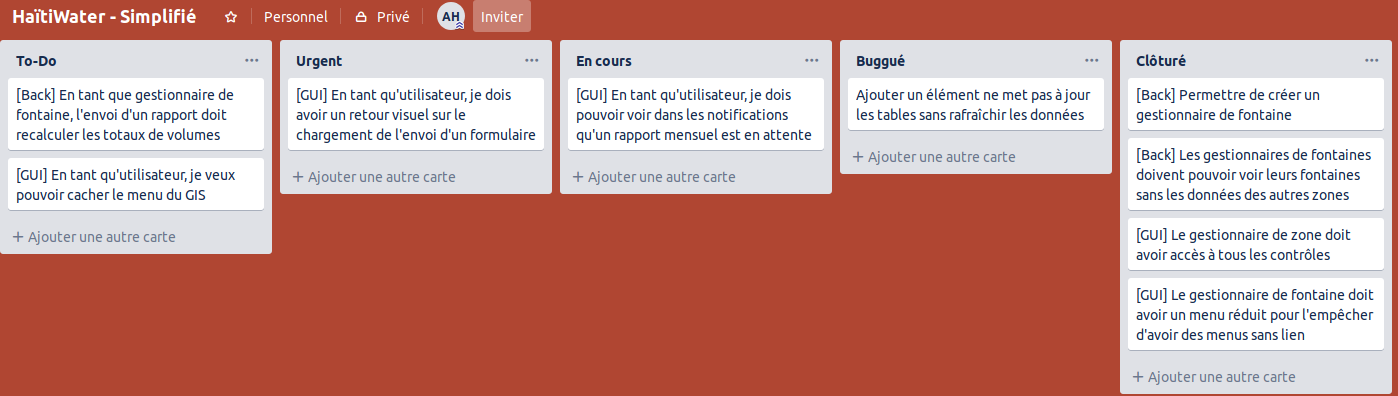
\includegraphics[width=\textwidth]{images/screen_trello_simplifie}
					\caption{Exemple simplifié d'interface Trello}
					\label{fig:screen_trello_simplifie}
				\end{figure}

				Etablir un plan et s'y tenir n'était cependant pas suffisant. Le projet a connu de nombreuses modifications dans ses objectifs et contraintes. Différents facteurs viennent expliquer ces modifications :

				\begin{itemize}
					\item La présentation de prototypes aux partenaires et aux promoteurs ont souvent amené de nouvelles idées pour l'application, ou suggéré la modification de fonctionnalités existantes.
					\item L'arrivée de nouveaux acteurs, principalement aux mois de février et mars. Plusieurs Haïtiens ont pu apporter des éclaircissements sur la situation qui ont modifié l'application et l'orientation de son développement.
					\item Certaines fonctionnalités se sont révélées plus complexes à implémenter que prévu.
				\end{itemize}

				La figure~\ref{fig:simplified_gantt} présente une vue simplifiée du diagramme de Gantt~\footnote{Un diagramme de Gantt présente l'avancement et les prévisions des tâches d'un projet en fonction du temps.} final sur lequel les modules implémentés (voir section~\ref{sec:cahier_des_charges}) sont placés sur une ligne temporelle en dessous de laquelle les grandes phases du mémoire ont été placées, ainsi que les deux versions majeures, \emph{alpha} et \emph{beta}, présentées à tous les acteurs du projet.

				Les phases d'\emph{analyse} et \emph{architecture} se sont également clôturées par des réunions de taille plus importante afin qu'un maximum de personnes puissent donner leur avis sur les artefacts (cahier des charges, ébauches d'interface graphique, etc). C'est notamment après ces réunions que les changements de planification étaient décidés pour répondre aux nouveaux besoins du client.

				Le diagramme en figure~\ref{fig:simplified_gantt} est donc la version finale. Comparé au plan initial, on constate une augmentation de la phase d'implémentation en raison de l'augmentation de la charge de travail, les modules \emph{historique} et \emph{finances} étaient en effet imprévus. De nombreuses autres fonctionnalités ajoutées a posteriori ont allongé cette phase.
				Il était également prévu de passer plus de temps sur l'analyse et la conception du système. Or le cahier des charges et les ébauches n'étaient pas assez concrets pour avoir des retours précis sur l'outil. Devant ce fait et l'ampleur du projet, nous avons démarré l'implémentation plus tôt que prévu, et elle s'est également allongée sur le mois d'avril (pour un total d'environ 6 semaines supplémentaires).

				Ces imprévus n'ont heureusement pas eu d'impact sur la production. Le démarrage anticipé de l'analyse en août, l'ajout d'une semaine de travail imprévue durant la session d'examen de janvier ainsi qu'une zone tampon de deux semaines prévue dans l'horaire initial ont permis d'accomplir la totalité des tâches initialement prévues, ainsi qu'une part appréciable des suggestions apportées au cours de l'année.

				\begin{figure}[H]
					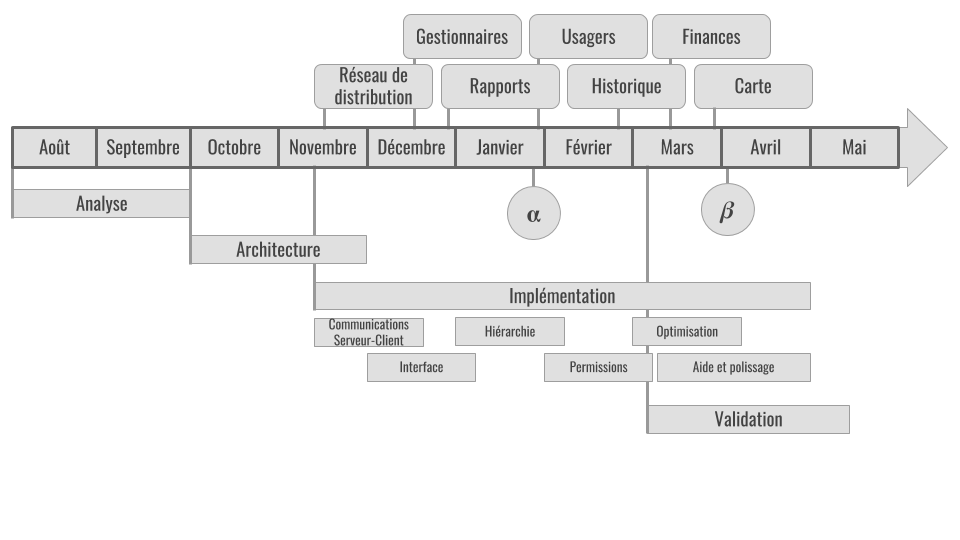
\includegraphics[width=\textwidth]{images/planning_timeline.png}
					\caption{Représentation simplifiée du diagramme de Gantt final}
					\label{fig:simplified_gantt}
				\end{figure}


			%\subsection*{Réunions}
			%(Adrien) Finalement je vois pas l'utilité de cette section "réunions"
			% (Seb) ça me semble pas utile non plus, on a déjà pu en parler suffisamment dans les autres sous-sections. À moins qu'on revienne plus en détail sur ce que nous avons pu montrer à Protos lors des deux réunions avec et ce qui en es ressorti ? pas sûr que ce soit vraiment utile.
			% Je pense qu'ici on s'étale déjà pas mal, en effet. On peut garder en mémoire que s'il faut couper, on peut le faire ici ;)

		\section{Méthodologie}

			Garantir l'avancement sans variation indésirable de tout projet se fait par le biais d'une méthodologie~\cite{ref:kolp_methodologies}. Il est important que cette méthode de travail soit connue de chacun pour garantir un rôle fixe et un suivi efficace. Cette notion de méthode est une caractéristique bien connue de la gestion de projet, le but étant de partir d'un besoin et d'apporter une solution informatisée. La méthode lie ces deux états et définit un système de communication, échéances, tâches, etc. De nombreuses méthodes déjà établies existent et sont prêtes à l'emploi par n'importe quelle équipe.

			\subsection*{Agile}

				Dans la section précédente, nous avons évoqué les changements constants dans la planification et les tâches. C'est donc tout naturellement que nous avons opté pour une \emph{méthode agile}, en opposition aux méthodes traditionnelles dites \emph{waterfall} qui se montrent plus rigides et réfractaires au changement.

				Nous n'avons pas suivi une méthode agile fixe, préférant une version plus relaxée, adaptée aux variations de disponibilité inhérentes à notre statut d'étudiant. On peut cependant relever des grands principes inspirés de méthodes existantes, notamment Scrum~\cite{ref:scrum}.

				\begin{description}
					\item[Développement dirigé par les fonctionnalités] \emph{Feature Driven Development} en anglais, ce type de développement focalise les ressources sur la création. Tout d'abord création d'un prototype général et d'une liste de fonctionnalités. Ensuite création de celles-ci, ajoutées à l'application en impliquant le client à chaque fois qu'une fonctionnalité est créée. C'est également le client qui définit la priorité des fonctionnalités. Ce dernier point fut très utile dans notre mémoire où les acteurs haïtiens ont souhaité orienter le développement vers l'aspect financier de l'application, en opposition à Protos qui accentuait principalement le réseau de distribution.

					\item[Itérations courtes] Une itération est une étape indépendante du développement. Chaque itération a sa propre planification et rétrospective. En méthode agile, les itérations sont courtes. Puisque nous voyions nos promoteurs toutes les semaines en alternance, nos itérations se sont naturellement calquées sur ce rythme. Nous avons évoqué l'intérêt de recentrer le développement en section~\ref{sec:planification}. C'est également une excellente manière de détecter rapidement les risques (tant au niveau de la planification que de l'application produite) et d'agir en conséquence.

					\item[Livraison continue] A partir de février, un acteur haïtien arrivé en Belgique a utilisé intensivement l'application. Grâce à ses retours, nous avons pu modifier l'application. Durant trois mois, nous avons déployé de nouvelles versions de l'application toutes les deux ou trois itérations afin qu'il puisse essayer les fonctionnalités ajoutées. Cela a nécessité un peu plus de travail, pour déployer l'application et garantir l'intégrité des données entre les différentes versions. Effort récompensé par des retours fréquents de la part d'un utilisateur impliqué dont le point de vue extérieur s'est avéré extrèmement utile.
				\end{description}

			\subsection*{Phases du mémoire}

				Si le développement (implémentation) de l'application a suivi ces principes agiles, on notera que le déroulement d'ensemble du mémoire est divisé en grandes phases. Ce principe est mis en avant dans la figure~\ref{fig:simplified_gantt}. Cette caractéristique est traditionnellement indicatrice d'un développement en cascade où les différentes étapes du développement logiciel sont délimitées en temps et responsabilités (analyse, conception, implémentation, test, déploiement).

				Les raisons sont multiples. On citera notamment notre méconnaissance des contextes de la gestion de l'eau potable et d'Haïti pour lesquels il a fallu se documenter pendant une période assez longue ainsi que la quantité de documents initiaux qui ont forcé à travailler durant ces premiers mois sur la compréhension et l'ébauche d'une solution.

				Les disponibilités des acteurs externes au développement (membres de Protos, Haïtiens, chercheurs externes) ont aussi été un facteur. Chacun ayant une mission déterminée, nous ne pouvions avoir de contacts trop fréquents (aussi dûs à la distance et au décalage rendant difficile l'organisation de réunions). Nous avons donc dû aussi adapter les itérations aux disponibilités, variables, de chacun. Ceci explique aussi partiellement pourquoi le développement s'est autant accéléré lorsque des acteurs haïtiens sont venus en Belgique et nous ont offert des retours fréquents, ont participé à différentes réunions. La disponibilité du client est très importante dans le développement agile afin de pouvoir évaluer le travail accompli. En l'absence de membres extérieurs, ce sont nos promoteurs qui ont parfois joué ce rôle de client.

		\section{Répartition des tâches}

			Dès le début, nous avons cherché à tirer avantage de nos centres d'intérêts et capacités différents. Nous avons eu la chance d'être une équipe complémentaire et d'avoir un mémoire intéressant au point que toutes les tâches étaient attribuées sans problème et rapidement. Dans cette section, nous discutons de cette attribution systématique et de ce qu'elle implique pour ce travail.

			\subsection*{Analyse}

				La phase d'analyse principale, d'août à octobre, avait pour but de comprendre la situation et le rôle de l'application. Afin que toute l'équipe avance vers le même objectif, il a été nécessaire que chacun soit impliqué dans l'analyse. En débutant par une recherche libre, nous avons cherché à nous documenter sur le contexte haïtien, les solutions existantes et les entreprises qui appliquent ces solutions. L'apport de plusieurs centaines de pages de documentation par Protos et nos promoteurs a nécessité une certaine organisation. Demander à chacun de nous, mémorants, de tout lire nous a semblé improductif, mais il était nécessaire que les informations circulent. Nous avons donc adopté un système de file pour les documents. Chaque nouveau document~\cite{ref:resumes_documents} est placé dans cette file et pris en charge par un de nous trois (selon disponibilité et affinité). Au fil de la lecture, un document résumant le contenu et relevant les informations utiles pour le mémoire est produit. Le résumé terminé et mis à disposition, il est lu et discuté en groupe. Un autre objectif de ce système est de pouvoir bénéficier de documents raccourcis pour rechercher des informations, notamment dans la rédaction de ce travail.

				Précisons cependant que même si ce que nous considérons être comme la phase d'analyse principale s'est déroulée de août à octobre, les changements d'exigences et l'apport de nouvelles informations au cours de l'année ont induit des phases d'analyse complémentaires, principalement au démarrage l'implémentation de chaque module. A nouveau, nous nous sommes tous trois impliqués dans ces phases afin que le développement aille dans un sens unique.

			\subsection*{Conception et implémentation}

				Contrairement à l'analyse, la conception et l'implémentation ont connu une très forte séparation des tâches entre nous trois, chacun ayant un champ de travail défini.

				\begin{description}
					%(Adrien): assez schématique pour le moment, à voir si on détaille en profondeur ? ça me semble pas hyper utile mais peut-être que les promoteurs vont vouloir plus de précision. Vous êtes invités à reformuler votre responsabilité si souhaité :) (ps: j'ai fait par ordre alphabétique des prénoms).
					\item[Adrien] responsable de la gestion du projet (planification, présentations intermédiaires, communication), de l'analyse fonctionnelle et du \emph{front-end} (le client) : interface graphique, fonctionnalités utilisateur.

					\item[Céline] responsable du \emph{back-end} (le serveur) : base de données, traitement des informations et calculs, gestion des performances.

					\item[Sébastien] responsable du \emph{service worker} (l'accès hors-ligne à l'application), des tests et renfort au \emph{back-end} sur le module financier et la vérification des permissions.
				\end{description}

				Pour chacune de ces préoccupations, le responsable désigné s'est chargé de la conception, des schémas, de la réalisation (implémentation) et de la documentation. Une communication constante et présentation de l'avancement des tâches à chaque membre de l'équipe se sont implicitement imposées, toujours dans l'optique d'orienter le développement dans le même sens.

				L'inconvénient principal de ce type d'organisation est la compartementalisation qui nuit à l'apprentissage individuel puisque tout le monde ne travaille pas avec la totalité des technologies utilisées. Cela pose un risque d'arrêt, même temporaire, du développement si un des membres se trouve dans l'incapacité d'assumer sa charge de travail. En entreprise, ce risque serait à corriger au plus vite en impliquant plus d'acteurs dans chaque branche du développement, ou en impliquant tous les acteurs dans la totalité du code (par exemple via un système de rotation).

				Nous avons tout de même effectué ce choix pour la puissance de travail qu'il permet et les facilités de développement et d'organisation apportées. Chacun de nous a développé une connaissance accrue de la technologie utilisée dans sa partie, permettant une augmentation drastique de l'efficacité qui s'est particulièrement ressentie dans la seconde partie (second quadrimestre) du travail. Organisationnellement parlant, savoir directement à qui s'adresser en cas de problème ou demande de fonctionnalité a été également particulièrement pratique.

			\subsection*{Rédaction}

				La rédaction du présent texte a à nouveau rassemblé l'équipe. En tant que document résumant et justifiant le travail accompli, il était naturel d'être tous inclus dans son élaboration. Nous avons considéré les différentes sections en tant qu'entités individuelles, permettant un déroulement de la rédaction simplifié, étape par étape. A des granularités différentes (parfois allant jusqu'à établir le plan pour chaque sous-section), nous avons dressé une liste du contenu à intégrer. La section était ensuite attribuée au mémorant responsable du sujet discuté.

				Une fois le premier jet établi, une relecture permettait à chacun d'apporter les modifications désirées, parfois discutées, pour obtenir un texte dans lequel chacun de nous peut s'identifier. Ce processus était répété pour chaque section et chaque jet, encouragés et orientés par les commentaires de nos promoteurs.

			\subsection*{Au quotidien}

				La planification générale avait une précision au maximum hebdomadaire. Pour le travail effectué au jour le jour, nous nous sommes entièrement reposé sur Trello avec un système de colonnes décrivant l'état et la priorité de chaque tâche comme exposé ci-avant. Autre héritage des méthodologies agiles, ces cartes sont des tâches à réaliser pour avancer le développement. Dans notre cas, les tâches étaient souvent atomiques ou ne reflétaient qu'une seule unité de développement (e.g., ajouter un champ dans un formulaire).

				Un système de description de la tâche, assignation de membre(s) à une carte et étiquetage, ajouté au principe des différentes colonnes indiquant la priorité et l'état de chaque carte, a permis de gérer efficacement le travail.

				Quant à l'ajout des cartes, on relève deux possibilités :
				\begin{itemize}
					\item Au début des itérations, lorsqu'on planifiait le sprint à venir.
					\item Durant une itération, lorsqu'un membre de l'équipe avait besoin d'une fonctionnalité qu'un autre membre devait implémenter, le premier membre ajoutait une carte en assignant le second. Par exemple, si le développement du client nécessitait l'implémentation d'une fonctionnalité du serveur, la carte était ajoutée en assignant directement la personne responsable.
				\end{itemize}

				La colonne de travail prioritaire s'est avérée une très bonne idée. Puisque nos fonctionnalités sont dépendantes à la fois du client et du serveur, cela permettait d'identifier clairement les besoins. Nous pouvions ainsi débuter une séance de développement à n'importe quel moment en sachant ce dont les autres avaient besoin.



	\chapter{Analyse des besoins}
		\label{sec:analyse_besoins}
		%Total des pages : 6 à 10
		La phase d'analyse des besoins est, dans tout projet, l'une des plus importantes. Elle se doit d'être méticuleuse, afin que tous les partis soient d'accord sur ce qu'ils souhaitent. Cependant, nous devions rester conscients que le temps accordé à un mémoire est assez court par rapport à ce qui se fait dans l'industrie pour un projet de cette taille. Nous ne pouvions donc pas passer trop de temps sur cette phase, sous peine de ne plus en avoir assez pour implémenter les fonctionnalités établies.

		Nous pensons avoir trouvé un bon entre-deux, prenant avantage des conseils glanés au cours de nos études~\cite{ref:kim_coo} : nous avons présenté au plus vite des visuels de la future application, et avons organisé une réunion Skype pour pouvoir échanger en direct avec nos clients malgré le déclage horaire.

		Le cahier des charges résultant de ces interactions nous semble complet, et a été assez peu modifié au cours du projet. Deux éléments s'y sont cependant ajoutés, l'un pour répondre aux besoins non-fonctionnels et l'autre suggéré par Louis Fritzno, un acteur haïtien venu pour apporter un point de vue concret.

		\section{Besoins fonctionnels}

			%Pages : 1 à 2
			Le terme \emph{besoins fonctionnels} décrit les besoins précis d'un client, les non-négociables dans le cadre d'un projet. Ce sont les points qui ont été mis en avant par Protos et les Haïtiens comme étant essentiels, nécessaires afin que notre application leur soit utile.

			\subsection*{Gestion des données}
				La chose la plus évidente dont ont besoin les acteurs sur place est une aide à la gestion de leurs données. La technique papier-crayon décrite plus tôt s'est montrée inefficace, il faut donc un système permettant à la fois de centraliser les données et d'éviter les pertes, tout en ne s'éloignant pas trop de ce que les Haïtiens connaissent et font aujourd'hui, afin que la transition vers le nouveau système informatisé puisse être facilitée par une certaine familiarité.

				Pour mieux comprendre la nature exacte des données en question, nous avons étudié des fichiers Excel~\cite{ref:resumes_documents}, qui servent à ce jour de premier pas vers une informatisation de la gestion du réseau de distribution d'eau.

				\begin{figure}[ht!]
					\centering
					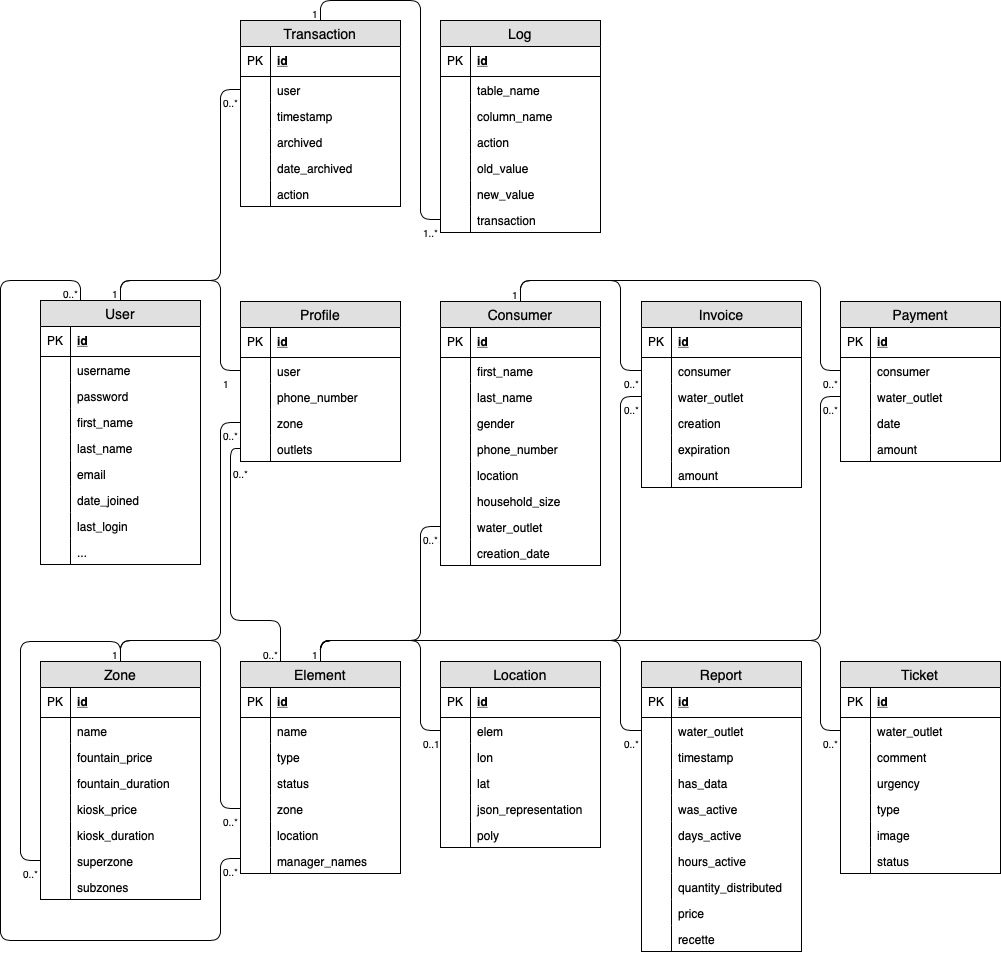
\includegraphics[width=\textwidth]{images/db}
					\caption{Schéma des données du système}
					\label{fig:db}
				\end{figure}

				Ces documents nous ont été d'une très grande utilité, puisqu'ils nous ont permis de lister toutes les données nécessaires à notre application, nous donnant un solide point de départ pour notre base de données. Nous en avons retiré une structure de données présentée dans la figure~\ref{fig:db}. Ils nous ont également permis de mieux comprendre quelles étaient les responsabilités des différents acteurs, ce qui nous a donné la structure de l'application elle-même.

				En nous inspirant directement des \emph{Komité Dlo} décrit dans le chapitre \ref{sec:structure_haiti}, nous avons décidé de créer deux types de gestionnaires : ceux dits \emph{de zone}, avec peu d'interaction avec les usagers du réseau, qui ont une vision plus globale de celui-ci. Ils collaborent avec des gestionnaires dits \emph{de fontaine(s)}, qui gèrent directement un ou plusieurs points d'eau, et sont en contact avec les consommateurs.

				Cette division permet à chacun d'avoir un rôle clair et précis, les gestionnaires de fontaines apportant les données au jour le jour (paiements, nouveaux usagers, etc.), tandis que les gestionnaires de zones s'occupent du réseau en lui-même.

			\subsection*{Simplification des procédures}
				La seconde observation que nous avons pu mettre en avant en lisant les documents fournis par Protos et en parlant aux Haïtiens est que les procédures en place sont à la fois trop compliquées et peu standardisées. Il est souvent nécessaire de se déplacer physiquement jusqu'à un point d'eau ou chez la personne qui en est responsable pour avoir l'information nécessaire, ce qui est à la fois une cause directe et un résultat de l'absence de centralisation.

				La division en différents rôles que nous avons établie permet aux utilisateurs de l'application d'avoir toujours une vue sur les éléments du réseau de distribution dont ils sont responsables, et de faire circuler les informations beaucoup plus vite.

				Nous souhaitons également aider les gestionnaires de zone à prendre des décisions plus rapidement. En effet, grâce à la numérisation des données, il leur est possible de visualiser leur réseau de distribution avec des filtres. Ceux-ci peuvent mettre en avant les points d'eaux nécessitant une réparation, ou les villages dans lesquels les factures sont en retard.

				%Je vois rien d'autre perso ?
				%non plus

		\section{Besoins non-fonctionnels}

			%Pages : 1 à 2
			Le terme de \emph{besoin non-fonctionnel} désigne un besoin caractérisant le système, une contrainte liée à l'implémentation, aux performances ou à une situation spécifique au projet en lui-même. Si ces buts ne sont pas atteints, l'application est quand même utilisable, leur réalisation est cependant nécessaire pour obtenir un système fiable et qualitatif.

			\subsection*{Sécurité des données}
				Dans le monde d'aujourd'hui, il est évident qu'une certaine attention se doit être accordée à la sécurité d'une application web. En Haïti peut-être plus qu'ailleurs, une attention particulière se doit d'être portée à la possibilité qu'un utilisateur malveillant ou non se connecte au système.

				Par conséquent, nous avons non seulement implémenté un principe de connexion avec privilèges (certaines données sont inaccessibles sans un niveau de privilège particulier), mais nous avons également ajouté un système de \emph{logs}.

				Ce module, appelé \emph{module historique} n'était pas prévu initallement, nous l'avons ajouté pour remédier aux erreurs des utilisateurs, ou aux comportements malicieux. Ce module permet aux supérieurs hiérarchiques de consuleter les modifications faites par leurs subordonnés. Si ces modifications leur semblent incorrectes, un seul clic leur permet de faire revenir les données à leur état précédent. Si une modification est acceptée, elle disparaît de la liste en laissant la modification, jugée valide, dans la base de données.

			\subsection*{Connexions lentes et peu fiables}
				L'utilisation de notre application en Haïti amène un besoin particulier : dans ce pays, la connexion Internet est bien plus lente que nos standards européens et y est souvent peu fiable. Pour pallier à cela, nous avons d'abord utilisé les techniques courantes : nous envoyons aussi peu de données que possible, faisons usage de la cache~\ref{sec:cache_client} et envoyons les informations des différents éléments de la page séparément.

				Cependant, une demande de nos clients a été de pouvoir utiliser certaines fonctionnalités de l'application lorsqu'il n'y a pas de connexion. Pour cela, nous avons développé un \emph{service worker}, détaillé en section~\ref{sec:service_worker}.

			\subsection*{Technologies simples et populaires}
				% Est-ce que c'est pas un besoin non-fonctionnel aussi ?
				Par rapport à un projet classique, une contrainte de ce travail est qu'il se déroule dans le cadre d'un mémoire universitaire. À la fin de nos études, ce projet sera repris par d'autres étudiants pour un deuxième mémoire et à terme il sera déployé en Haïti pour être maintenu par les acteurs locaux. Comme ces futurs développeurs ne sont pas connus, une attention particulière doit être apportée à la facilité de la maintenance de notre application.

				Pour cela, nous avons décidé d'utiliser des technologies relativement simples et populaires, de sorte que même si nos successeurs ne les connaissent pas ils puissent assez facilement les apprendre par eux-même, en utilisant des tutoriels disponibles gratuitement sur internet par exemple. Une description plus détaillée des choix technologiques que nous avons fait se trouve à la section~\ref{sec:choix_tech}.

		\section{Cahier des charges}
			\label{sec:cahier_des_charges}

			% Important : dans cette section, il faut impérativement parler des modules.
			% Expliquer que le besoin non-fonctionnel d'évolutivité de l'application justifie l'utilisation de "modules". Expliquer comment ils s'intègrent en un seul système, et puis donner un résumé, pour chaque module, de ce qu'il permet de faire.
			% Et en fait c'est le seul endroit où on peut parler de tout ça, donc ça doit être fait ici.
			%Pages : 2 à 3
			Après discussion avec Protos et les Haïtiens, nous avons décidé d'organiser notre application en différents modules indépendants intéragissant avec notre base de données. Ce choix de conception nous a permis dans un premier temps d'appliquer la méthode Agile plus facilement, déployant notre travail module par module. Dans un second temps, il permet à notre application d'évoluer très rapidement : un nouveau module vient se greffer à la base de donnée sans changer le fonctionnement des autres, un ancien module qui aurait perdu son utilité peut être enlevé sans rien endommager. De plus, ce choix devrait aider les futurs développeurs à ajouter à la base applicative existante plus rapidement.

			Chaque module représente un type d'activité pratiqué par les gestionnaires du réseau de distribution. Après cette première année de développement, nous en avons créé huit :
			\begin{itemize}
				\item Le module \textbf{réseau}, permet de créer de nouveaux éléments du réseau (source, conduite, réservoir, kiosque, fontaine, prise individuelle) et de consulter des informations à leur propos (nom, emplacement, état de fonctionnement)
				\item Le module \textbf{carte interactive}, fortement lié avec le précédent, permet de placer et visualiser les éléments du réseau de distribution sur une carte. Le module permet de placer des éléments au jugé avec la souris, ou directement avec trois systèmes de coordonnées : le degré décimal, le degré-minute-seconde et la transverse universelle de Mercator (cette dernière méthode demandée par notre contact haïtien).
				\item Le module \textbf{consommateurs} contient toutes les informations à propos des usagers du réseau (nom, adresse, etc), groupés par ménages.
				\item Le module \textbf{financier}, fortement lié avec le module précédent, permet de consulter et d'ajouter les informations concernant les paiements réalisés par les usagers du réseau.
				\item Le module \textbf{rapports} permet aux gestionnaires de fontaine(s) d'entrer des informations sur le fonctionnement du réseau (s'il a été actif, quelle quantité d'eau a été distribuée) et de créer des tickets de problèmes en cas de panne d'un élément.
				\item Le module \textbf{gestion de zone}, plus administratif, permet de créer de nouveaux gestionnaires et de les assigner à une zone ou des éléments du réseau en fonction de leur rôle.
				\item Le module \textbf{historique} permet aux supérieurs hiérarchiques de visualiser tous les changements, ajouts ou suppressions effectués par leurs subordonnés. Ils peuvent valider ou annuler ces changements. Pendant trois semaines, un choix (validation ou annulation) est affiché dans une seconde table pour informer les autres supérieurs qu'une décision a été prise, voire de récupérer des informations supprimées en cas d'annulation erronée.
				\item Le module \textbf{offline} permet d'assurer la disponibilité du site même lorsque la connexion internet n'est pas stable, donnant la possiblité de compléter le rapport mensuel.
			\end{itemize}

			%\subsection*{Complet en annexe ?}

		%\section{Structure des données}

			%Pages : 2 à 3

			%\subsection*{Complet en annexe ?}

	\chapter{Implémentation}

		Total des pages : 16 à 22
		% Auteur : Adrien (+Seb)
		% Relu :  Céline

		% L'implémentation suit les principes du cahier des charges. Intègrer les fonctionnalités demandées et respecter les besoins du client.

		\section{Choix technologiques}
			\label{sec:choix_tech}

			Pages : 3 à 4
			% Outils informatiques, plusieurs choix, le notre n'est pas le meilleur mais celui qui nous a semblé le plus adapté.
			% Ici on détaille les choix majeurs. Les bibliothèques plus petites sont détaillées dans la documentation.
			% Ici, donc, uniquement ce qui est soit réellement gros, soit souvent utilisé

			% Expliquer le trade-off constant entre les techs choisies

			% TODO figure montrant un visuel sur l'architecture choisie

			\subsection*{Web}
				% Requis du client. Avantage de la portabilité, installation, données décentralisées directement, donc communes à tous les utilisateurs
				% Désavantage support des navigateurs multiples, perte en performances d'opérations complexes, nécessite plus de bande passante, rend plus difficile l'accès hors-ligne aux fonctionnalités

				\'Etablie dès le premier jour, l'exigence du support web pour ce travail a influencé la totalité du mémoire. Nous n'avons pas eu de réel choix à ce niveau, il nous est néanmoins possible de trouver des avantages à ce type de développement :
				\begin{itemize}
					\item L'application ne nécessite aucune installation, aucun prérequis et la seule nécessité est de disposer d'un navigateur internet (préférentiellement majeur et relaivement récent). C'est une facilité pour l'utilisateur, puisqu'il suffit d'accéder au site internet. L'avantage est également étendu au développement qui ne doit pas se préoccuper du système d'exploitation de l'utilisateur.
					\item Le déploiement des mises à jour et la manière dont l'application fonctionne en général est uniforme à travers les utilisateurs et les conflits de version, bien que devant toujours être gérés notamment par le biais du cache (voir section~\ref{sec:cache_client}), sont moindres que sur une application locale. D'éventuels conflits de données peuvent être réglés directement via le serveur et les outils de développement disponibles à l'équipe, ce qui est plus rapide et moins complexe que de créer des automatisations pour gérer ces mises à jour individuellement pour chaque utilisateur.
					\item
				\end{itemize}

				Ne présentant pas que des avantages, le développement web apporte son lot de problématiques nouvelles :
				\begin{itemize}
					\item Utiliser une application en ligne nécessite une connexion internet, et même si cette dernière n'est pas requise en permanence (voir section~\ref{sec:service_worker}), il est impératif qu'elle soit présente ponctuellement pour charger l'application et envoyer/recevoir les données lors de son utilisation.
					\item La diversité des navigateurs internet (Firefox, Chrome, Edge, etc) entraîne la nécessité de gérer ces environnements différents pour que l'application fonctionne sur un maximum de navigateurs et de manière similaire.
					\item
				\end{itemize}

			\subsection*{Choix du framework - Django}
				% Framework éprouvé (ancien, maintenu, communauté, documentation), adapté à de larges applications (scalable), permet l'utilisation facilité de PostgreSQL (modèles), gabarits pour du HTML 'importé' sans besoin d'angular/whatever (moins de techs, reste simple).

				Un framework est une infrastructure logicielle dans laquelle l'application est développée. On peut argumenter, avec raison, qu'un framework ajoute une certaine quantité d'outils qui ont pour effet de complexifier l'application et d'en augmenter la taille. Dans une application aussi large que la nôtre cependant, l'apport bénéfique qu'ont ces outils supplante largement ces inconvénients. Parmi ces apports bénéfiques on citera surtout :
				\begin{itemize}
					\item L'environnement de travail d'un framework impose certaines contraintes qui répandent des bonnes pratiques. Par exemple une structure des fichiers du code source qui permet à long terme une meilleure maintenance, surtout dans de larges applications.
					\item Les outils fournis sont testés, utilisés et éprouvés. Il n'est pas nécessaire de créer nous-même des fonctionnalités déjà présentes dans un framework, et même si recréer ces fonctionnalités est une expérience enrichissante, elle reste moins efficace. De plus, les fonctionnalités existantes sont de meilleure qualité, offrent de meilleures performances et surtout ne sont pas à maintenir par l'équipe de développement de l'application, mais par l'organisme en charge de la publication du framework. Ces avantages seront d'autant plus importants que le framework est populaire et maintenu à jour.
					\item Un framework aura beaucoup de fonctionnalités par défaut qui rendront le développement plus aisé. Messages d'erreur, outils de mesures, etc.
					\item La documentation et l'aide sont de meilleure qualité. Les framework ont généralement une communauté et une équipe de développement dont les capacité et l'expérience permettent une production de documentation rendant très facile la compréhension du projet et la recherche d'aide. Avantages qu'il est impossible d'égaler dans une équipe de trois personnes sur dix mois.
				\end{itemize}

				La table~\ref{table:comparatif_framework} reprend une liste non-exhaustive de frameworks qui ont été envisagés pour ce projet. Afin de pouvoir développer une application compatible, nous avons évalué les possibilités et arrêté un choix durant la phase d'analyse du développement. Ci-après sont exposées les motivations de ce choix.

				\begin{table}[H]
					\centering
					\begin{tabular}{|c|c||c|c|c|c|c||c|}
						\hline
						\textbf{Langage} & \textbf{Framework} & \textbf{C} & \textbf{M} & \textbf{Pe} & \textbf{Po} & \textbf{T} & \textbf{Total} \\
						\hline
						\multirow{4}{*}{\textbf{JavaScript}} & Express & M & M & B & B & M &3.5 \\
						 & MeteorJS & B & B & M & N & B & 3.5\\
						 & NodeJS & M & M & M & B & N & 3.5\\
						\hline
						\multirow{3}{*}{\textbf{Python}} & Django & M & M & B & B & M& 3.5\\
						 & Flask & B & B & B & B & B & 5\\
						 & Pyramid & B & B & B & N & B & 4\\
						\hline
						\multirow{1}{*}{\textbf{Ruby}} & Rails & N & M & B & B & B & 3 \\
						\hline
					\end{tabular}
					\label{table:comparatif_framework}
					\caption{Comparatif de quelques frameworks connus}
				\end{table}

				\subsubsection*{Critères - [B]on, [M]oyen, [N]égatif}

					\begin{description}
						\item[C] Complexité - Difficulté d'utilisation / apprentissage. \hfill \\
							\'Evaluer la complexité est hautement subjectif en fonction des préférences et habitudes du développeur. Nous pouvons néanmoins comparer les langages utilisés et la structure du framework.

							Une mesure de la complexité se base sur l'imbrication des blocs de code. Un code comportant beaucoup de structures imbriquées sera moins lisible, et donc plus complexe. Les résultats\footnote{\'Etude de Seerene~\copyright, 2015} en figure~\ref{fig:complexity} montrent que cette mesure favorise le langage Python dans nos options.

							\begin{figure}
								\centering
								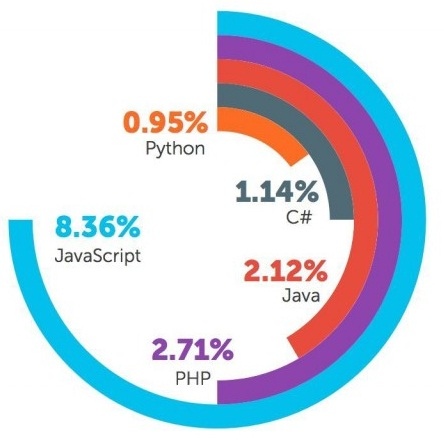
\includegraphics[width=.6\textwidth]{images/complexity}
								\caption{Pourcentage de code imbriqué}
								\label{fig:complexity}
							\end{figure}

					\item[M] Maintenabilité - Aisance et possibilités de maintenance. \hfill \\
							L'aisance avec laquelle un code est maintenu à jour est inversement lié à la complexité. \'A cela, nous pouvons ajouter les fréquences de mise à jour des frameworks. La structure du framework impacte également la maintenabilité ; moins on modifie de fichiers pour implémenter une fonctionnalité, plus facile sera la maintenance à moyen et long terme.

					\item[Pe] Performance - Capacités du framework. \hfill \\
							Bien que moins importantes que dans une application critique (e.g.: aérospatial, banque), les performances sont mesurées en termes de temps de réponse pour une requête du client au serveur.

					\item[Po] Popularité - Popularité du langage à travers le monde. \hfill \\
							La popularité est sans doute la plus importante des mesures de ce comparatif. Un langage populaire dispose de plus de tutoriels et aide en ligne que d'obscurs langages / frameworks peu ou pas utilisés.

							La figure~\ref{fig:hotframework}~\footnote{https://hotframeworks.com/} montre une évolution de la popularité des frameworks les plus courants.

							\begin{figure}
								\centering
								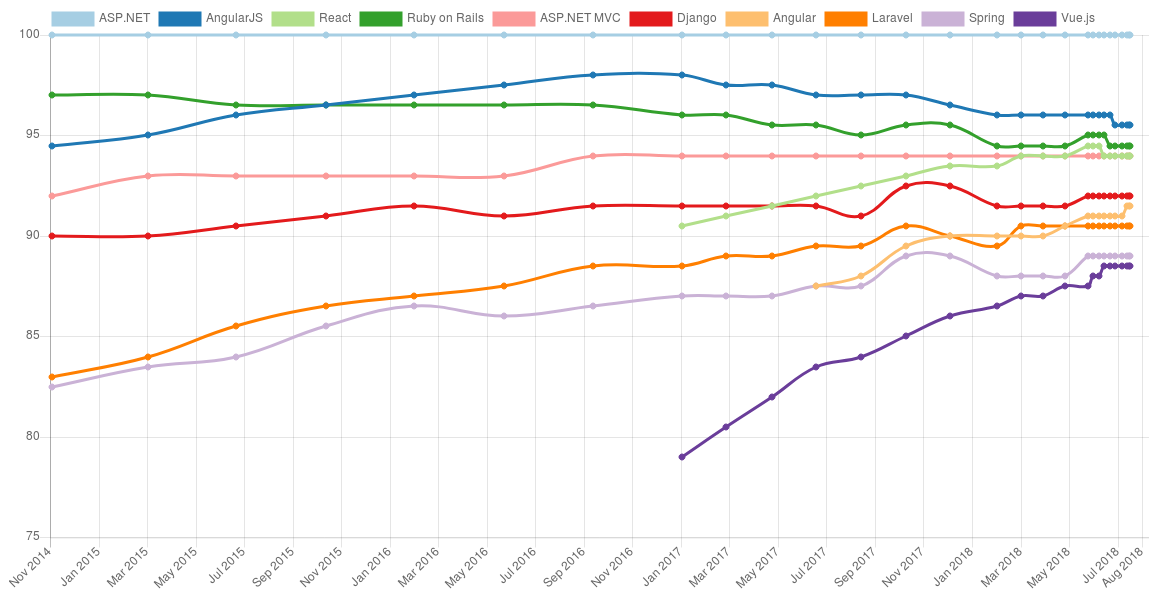
\includegraphics[width=\textwidth]{images/hotframework.png}
								\caption{Popularité des frameworks de novembre 2014 à août 2018}
								\label{fig:hotframework}
							\end{figure}

					\item[T] Taille - Espace de stockage requis \hfill \\
							Un framework léger sera plus intéressant pour ce projet. D'une part pour la complexité, car moins il est nécessaire de modifier/ajouter des fichier, plus l'utilisation est aisée. D'autre part car le serveur de destination nous est inconnu et nous ne savons donc pas quel espace de stockage sera mis à disposition.
				\end{description}

				\subsection*{Django}
					Le choix d'un framework repose sur de nombreux critères dont plusieurs sont subjectifs. En l'absence d'une ligne directrice, le choix se fait souvent selon l'expérience et les désirs de l'équipe. Notre comparatif terminé, il est devenu clair que nous favorisions un framework utilisant le langage de programmation Python.

					Flask a été envisagé, cependant les facilités offertes par Django dans la gestion de la base de données, particulièrement pour les données géographiques, ont été le facteur décisif. Parmi les sites populaires utilisant Django, on citera Instagram, DropBox, Disqus~\footnote{https://djangostars.com/blog/10-popular-sites-made-on-django/}.

			\subsection*{Python}
				% Obligé par Django, quand même un bon choix. Pas le plus répandu (PHP et ASP.NET bien plus utilisés) mais permet une bonne gestion des objets intégrée directement au serveur, car langage OO.
				Le langage Python est un langage de programmation populaire principalement grâce à sa syntaxe légère permettant un code compréhensible et généralement plus court (voir figure~\ref{fig:complexity}). Il n'est pas le plus utilisé, ce sont PHP (79\% d'utilisation), ASP.NET (11.3\%) et Java (4\%) qui constituent le trio de tête~\cite{ref:popular_programming_languages}. Toutefois, nous pensons que Python s'adapte parfaitement aux besoins de l'application demandée. C'est un langage relativement simple et compréhensible dont la popularité croît ces dernières années. Les bibliothèques logicielles et la documentation, toutes deux disponibles à foison sur internet, en font un langage particulièrement ouvert aux débutants. Un dernier argument, et non des moindres, est l'expérience déjà acquise dans la programmation en Python durant nos années d'études.

			\subsection*{PostreSQL et PostGIS}
				% Autre obligation de Django, mais une décision consciente de l'utiliser pour PostGIS. Manipulation géographique facilitée, un apport positif pour la suite du module GIS.
				% Petit comparatif d'utilisation des SGBD avec MySQL, etc ?
				% Pourquoi BDD relationnelle et non-relationnelle ?

				Si l'utilisation du langage Python était imposée dès lors que Django fut choisi en tant qu'environnement logiciel, le système de gestion de base de données, dont le rôle est de lier l'application web et la base de données, a pu être choisi un peu plus librement.

				Nous avons tout de suite écarté les systèmes non-relationnels. Bien que présentant des avantages, principalement dans l'agilité avec laquelle la structure des données peut évoluer, ces derniers ne sont pas adaptés à une application comme celle développée dans le cadre de ce mémoire. En effet, les données ont de fortes dépendances, les éléments du réseau étant rattachés à des gestionnaires faisant parties de zones géographiques elle-même gérées, etc. Les outils offerts par les bases de données relationnelles pour joindre différents groupes de données (par exemple pour croiser les consommateurs avec leurs paiements afin d'obtenir un détail financier), sont tout simplement mieux adaptés au fonctionnement de l'application.

				Restent donc les systèmes de gestion de base de données (SGBD) relationnels, dans lequels nous avons opté pour PostgreSQL, classé quatrième système de gestion de bases de données le plus utilisé au monde~\footnote{\url{https://db-engines.com/en/ranking}, 1 mai 2019}. La première motivation de ce choix est la recommandation du framework Django, lequel s'adapte mieux à ce SGBD via son système de \emph{mapping objet-relationnel} (voire section~\ref{sec:serveur}). La seconde motivation est l'existence de l'extension PostGIS~\cite{ref:postgis}, une extension du SGBD permettant de traiter aisément les données géographiques.

			\subsection*{Bootstrap}
				% Conventions connues (largement utilisées) pour le Front, beaucoup de choses pré-faites pour accélérer le développement.
				% Responsivité facilité grâce aux systèmes de base
				% Désavantage; un peu lourd en raison des fonctions non-utilisées, mais solution (lier la section améliorations futures où on va parler du cleanup des vendeurs)

				Bien que l'utilisation de frameworks \emph{front-end} soit de plus en plus répandue, nous n'en avons pas intégré dans le client de l'application. Les choix sont pourtant nombreux et tant Angular, React que Vue ont été envisagés. Nous avons décidé de n'en utiliser aucun pour ne pas ajouter de technologie supplémentaire et pour limiter le nombre de dépendances du projet afin d'en garantir la perrenité sur le long terme.

				Néanmoins, la version 3 (plus documentée, éprouvée et ayant de meilleures compatibilités avec les autres frameworks et bibliothèques que la version 4) de Bootstrap est présente dans l'application. Bootstrap est une bibliothèque implémentant une large quantité de fonctionnalités que nous utilisons majoritairement pour agencer visuellement les blocs de l'interface graphique en fonction de la taille de l'affichage disponible, afficher des composants avancés (multisélection, sélection de date, menus) et styliser les composants de l'interface.

				Bootstrap ajoute l'avantage non-négligeable d'implémenter un bon nombre de fonctionnalités nous permettant d'accélerer le développement, tout en étant une bibliothèque assez connue que pour être extensivement testée et documentée, la rendant une meilleure alternative à une création personnalisée qui aurait sans doute été moins performante.

				Le désavantage majeur est son poids. Accompagnée de nombreuses fonctionnalités qui n'ont pas été utilisées dans ce projet, Bootstrap est lourde (approximativement 400 KB), d'autant plus en considérant la lenteur des connexions haïtiennes,. Il est cependant tout à fait possible de nettoyer la bibliothèque (voir section~\ref{ref:suite_projet}) pour n'en conserver que les fonctionnalités utilisées, et ainsi optimiser les téléchargements.

			\subsection*{DataTables}
				% Un constat ; les tables Django ne permettent pas de contrôler l'information à 100%
				% Second constat ; on veut une API (référence serveur)
				% DataTable, librairie connue, avec un gros support, grosse documentation, beaucoup de modules pour gérer les tables, AJAX pour 100% séparer les données de leur présentation

				DataTables~\cite{ref:datatables} est la seconde plus grosse bibliothèque du projet, gérant l'affichage des données sous forme de tables. A nouveau sélectionnée de par son ancienneté permettant une documentation et des tutoriels efficaces, DataTables était très loin d'être la seule option. Nous avons envisagé, et débuté la première version avec, la bibliothèque \emph{Django-Tables2} qui causait un ralentissement du chargement des pages contenant les données, et une perte de contrôle de l'information au niveau du serveur car les tables étaient directement rattachées aux modèles de la base de données.

				Dans notre volonté d'offrir une API pour communiquer avec le serveur (voir section~\ref{sec:serveur}), nous avons migré vers DataTables. En utilisant la technologie AJAX (Asynchronous Javascript And XML) de DataTables, nous pouvons exploiter pleinement l'asynchronicité du navigateur et charger une page de l'application en totale indépendance des données, ce qui augmente la vitesse de chargement des contrôles, permettant d'utiliser directement une fonctionnalité de l'application sans attendre le téléchargement des données (par exemple pour ajouter un élément).

				Les capacités offertes par DataTables sur le contrôle des données nous permettent également de gérer les données à l'envoi et/ou à la réception et de contrôler leur affichage, tout en bénéficiant des fonctionnalités implémentées par la bibliothèque (champ de recherche, tri dynamique, pagination).

				Outre son poids conséquent auquel nous pouvons à nouveau opposer la solution évoquée dans la bibliothèque Bootstrap, DataTables requiert d'implémenter les fonctionnalités de l'API et de gérer le transfert et traitement des requêtes en envoi et réponse du client et du serveur, ce qui représente une charge de travail non-négligeable.

			\subsection*{Chart.JS}
			  % Présenter l'information visuellement.
				% Même avantage que DataTables, on envoie uniquement des données, tout se fait en front. Une des plus utilisées, mais pas la numéro 1 car D3.JS est un monstre, plus difficile à comprendre et utilise un système d'objets qui alourdissent considérablement la page, difficile de savoir si les périphériques haïtiens vont supporter. ChartJS utilise des canevas, plus légers. Moins dynamiques mais quand même certaines possibilités

				La bibliothèque Chart.JS est utilisée pour générer les représentations visuelles de l'application. Les bibliothèques permettant de créer des graphiques sont nombreuses et Chart.JS a de nombreux concurrents qui offrent parfois plus de fonctionnalités. Chart.JS a une bonne réputation dans ce domaine et est réputée pour ne pas être trop complexe à utiliser, toujours dans le but de respecter les exigences technologiques.
				De plus, Chart.JS génère des canvas là où un de ses concurrents majeurs, la bibliothèque D3.JS, génère des images vectorielles ou des éléments du domaine, plus gourmands en performances en particulier avec de larges ensembles de données.

		\section{La hiérarchie dans l'application}
			% Pages : 1 à 2
			% La base du foncitonnement d'HaïtiWater.
			% Deux types d'utilisateurs :
				% Gestionnaire de fontaine, le plus proche des consommateurs.
				% Gestionnaire de zone, supervision

			Le bon fonctionnement de l'application repose sur le principe hiérarchique de la récolte des informations venant de la saisie de données par les utilisateurs de l'application puisque le manque de financement et l'état actuel du réseau ne permet pas une récolte en temps réel des données via des capteurs. Une représentation de la structure hiérarchique vous est présentée en figure~\ref{fig:principe_hierarchique}.

			\begin{figure}[H]
				\centering
				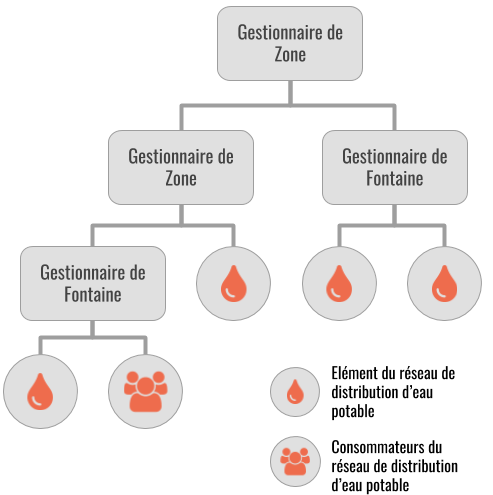
\includegraphics[scale=0.45]{images/principe_hierarchique}
				\caption{Représentation du principe hiérarchique des utilisateurs, éléments et consommateurs}
				\label{fig:principe_hierarchique}
			\end{figure}

			\subsection*{Structure}
				% Les utilisateurs s'organisent dans un système en arbre.
				% Noeuds : éléments du réseau, gestionnaires
				% Edges : lien de hiérarchie.
				% Seul le gestionnaire de zone peut avoir des enfants.
				% Aucune limite sur le facteur de branchement ou la profondeur de l'arbre

				% Système utilisé pour s'adapter partout à la configuration d'Haïti (exemple de DINEPA super-zone, OREPA zone lvl1, CAEPA zone lvl2, Comité fontaine a un gestionnaire de fontaine lvl3).
				% Permet d'avoir plusieurs niveaux de granularité. Par exemple si une région a besoin de plus de hiérarchie (si plus développée), on peut avoir plus de niveaux qu'une région qui en nécessite moins
				% Permet d'être réutilisée dans d'autres pays, structure simple à responsabilités définies

				% Point négatif qu'on repose entièrement sur les gestionnaires de fontaine pour avoir l'information (paiements, état du réseau, volumes). Mais c'est la seule possibilité vu que l'info ne peut pas être récupérée automatiquement.

				Rappelons que l'application a trois concepts clefs :
				\begin{description}
					\item[Zone] \hfill \\
						Une zone est un partitionnement des données de l'application. A la base de l'application se situe la zone racine dans laquelle toutes les données sont enregistrées. Une zone peut être composée d'autres zones. Une zone parente rassemble la totalité des données des zones filles. En revanche, une zone fille ne rassemble que les données qui lui sont rattachées et ne voit pas le contenu des zones soeurs. On peut ainsi se servir des zones pour diviser géographiquement le réseau de distribution d'eau selon le principe de la hiérarchie haïtienne existante (DINEPA, OREPA, CAEPA) exposée en section~\ref{sec:structure_haiti}. Chacun a donc ses propres responsabilités et ne vient pas empiéter sur le territoire de l'autre.
					\item[Elément du réseau] \hfill \\
						Un élément du réseau peut être une conduite, un réservoir, une source, une fontaine, un kiosque ou une prise individuelle. Ces six éléments constituent le réseau de distribution d'eau potable haïtien et sont enregistrés dans une zone.
					\item[Consommateur] \hfill \\
						Un consommateur est un habitant qui utilise le réseau de distribution d'eau potable. Dès son enregistrement dans l'application, le consommateur est rattaché à un élément de sortie (fontaine, kiosque ou prise individuelle) du réseau, ce qui permet de gérer sa facturation et, de manière plus générale, de consulter la densité des consommateurs.
				\end{description}

				Deux types d'utilisateurs sont amenés à se connecter à l'application :
				\begin{description}
					\item[Gestionnaire de Fontaine] \hfill \\
						Ce gestionnaire est un noeud terminal dans un chemin de la hiérarchie des utilisateurs. Son rôle est simple; au plus proche du consommateur, il est chargé de gérer (et donc assigné à) un ou plusieurs éléments de sortie du réseau, c'est-à-dire qu'il s'occupe du bon fonctionnement de la distribution aux consommateurs. Il a quatre charges relatives aux éléments du réseau de distribution d'eau qui lui sont assignés :
							\begin{enumerate}
								\item Rapporter l'utilisation, sous forme des volumes distribués.
								\item Signaler les problèmes avec la pompe ou avec la qualité de l'eau.
								\item Ajouter, modifier ou supprimer les consommateurs.
								\item Rapporter les paiements des consommateurs.
							\end{enumerate}
						Le gestionnaire de fontaine est donc une entité locale similaires aux \emph{comités fontaines} vus en section~\ref{sec:procedures_actuelles}.
					\item[Gestionnaire de Zone] \hfill \\
						Le gestionnaire de zone est un rôle plus complexe. Il est un administrateur local ou global, dépendamment de sa position dans la hiérarchie. Un gestionnaire de zone peut superviser d'autres gestionnaires, de zone ou de fontaine, et ce en nombre illimité. Un gestionnaire de zone peut effectuer les mêmes actions qu'un gestionnaire de fontaine, mais ses charges sont plutôt orientées dans l'administration  de sa zone:
							\begin{enumerate}
								\item Ajouter, modifier ou supprimer des zones.
								\item Ajouter, modifier ou supprimer des gestionnaires.
								\item Assigner des gestionnaires de zone à une zone, et des gestionnaires de fontaine à un ou plusieurs éléments de sortie du réseau.
								\item Gérer ses gestionnaires et leurs actions via l'historique.
								\item Utiliser les données récoltées par ses gestionnaires pour gérer le réseau de distribution.
							\end{enumerate}
				\end{description}

			\subsection*{Permissions}
				% Gestionnaire de zone; tout, dans sa zone et enfants.
				% Gestionnaire de fontaine; tous les droits sur la gestion des consommateurs et des paiements. Ne peut pas modifier le réseau ou les utilisateurs de l'application
				% On dispose quand même d'un garde-fou, le module d'historique
				Bien entendu, une hiérarchie implique un système de permissions. Dans notre application, ce dernier se calque exactement sur la structure exposée ci-avant. En toute normalité, les utilisateurs ne peuvent effectuer que les actions qui sont assignées à leur rôle. L'interface propose des contrôles réduits aux gestionnaires de fontaine, en opposition aux gestionnaires de zone qui doivent assumer leurs responsabilités supplémentaires.

				De plus, les données sont fortement liées à la hiérarchie et empêchent une quelconque utilisation, ajout, modification ou suppression par un utilisateur non-autorisé. Lorsqu'une donnée, peu importe son type (une zone, un consommateur, un rapport mensuel, etc), est ajoutée dans l'application, elle n'est visible que par l'utilisateur qui l'a créée et les utilisateurs qui lui sont supérieurs dans la hiérarchie (utilisateurs parents).

				En somme, plus un utilisateur est haut dans la hiérarchie, plus il a de pouvoir sur les données de l'application, la zone racine étant donc la somme de toutes les données, faisant des gestionnaires de cette zone les utilisateurs ayant le plus d'impact sur le système.

		\section{Interface utilisateur}
			% A fusionner avec "Client" ?

			% Pages : 2 à 3
			% La GUI n'est qu'une manière d'utiliser l'application. Pour l'instant la seule, mais on différencie vraiment le serveur et l'application car au final la webapp n'est qu'une GUI pour l'API.
			% Les fonctionnalités

			Partie visible de notre application, l'interface graphique, permet d'utiliser les fonctionnalités d'HaïtiWater. En réalité, l'interface graphique n'est qu'un moyen de faciliter l'utilisation de l'application et de rendre les données accessibles et lisibles par un humain. L'application est entièrement contrôlée par l'API qui requiert les données à afficher ou modifier. Somme toute, n'importe quelle autre interface (application locale, mobile, etc) pourrait envoyer les mêmes requêtes. Cela permet donc de décentraliser la logique de l'application dans le serveur tandis que l'interface permet de présenter l'information à un humain (tableaux, graphiques), le guider dans son utilisation et faciliter la saisie de données via les formulaires. Non content de permettre, dans le futur, la création de nouvelles interfaces, cette séparation des rôles nous a permis d'améliorer le développement et la maintenance de l'application, nous y reviendrons en section~\ref{sec:serveur}.

			Se voulant simple, l'interface est composée de blocs de contrôle permettant de gérer les données dans une zone de travail commune à toute les pages permettant de naviguer à travers l'application.

			\begin{figure}[H]
				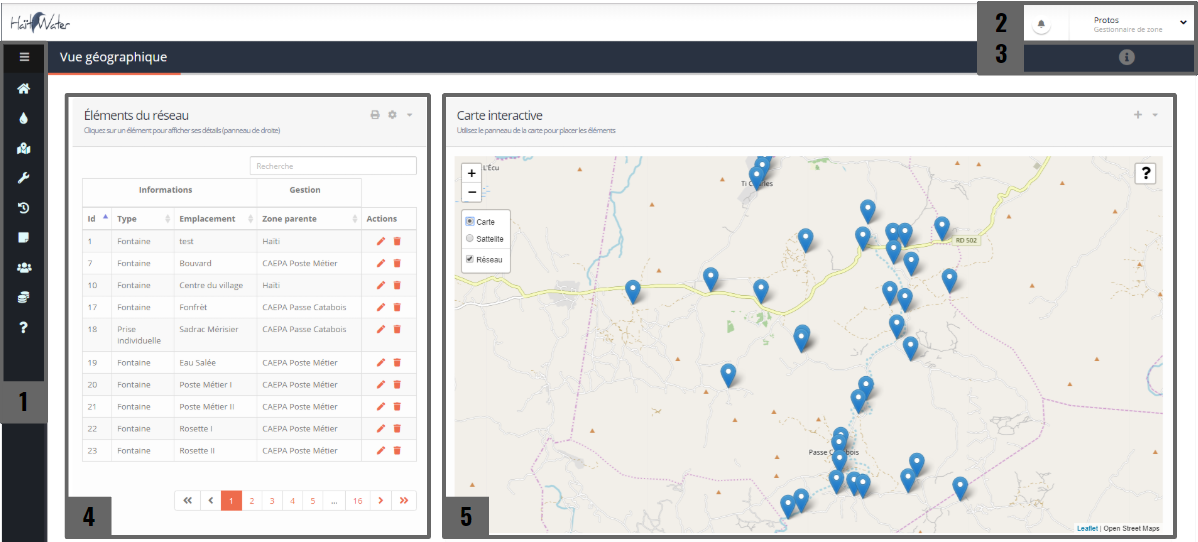
\includegraphics[width=\textwidth]{images/screen_gis_numbered.png}
				\caption{Capture d'écran du module géographique d'HaïtiWater}
				\label{fig:capture_gis}
			\end{figure}

			Une capture d'écran de l'application vous est présentée en figure~\ref{fig:capture_gis}. Les contrôles communs incluent :
			\begin{enumerate}
				\item Le menu déroulant permettant d'accéder aux modules de l'application.
				\item La zone utilisateur qui affiche ses notifications et le nom de compte qui lie à la déconnexion ou modification des informations personnelles dans son menu déroulant.
				\item L'aide rapide, permettant de déclencher une visite virtuelle de la page ouverte, visite textuelle qui présente brièvement les contrôles et leur utilité.
			\end{enumerate}

			Les contrôles spécifiques à cette page sont :
			\begin{enumerate}\setcounter{enumi}{3} % Reprendre à 3 pour suivre les labels du screen "fig:capture_gis"
				\item La table est un bloc de contrôle récurrent dans notre application. Ici listant les différents éléments du réseau de distribution, chaque table possède un champ de recherche, un système de tri et des contrôles permettant d'ajouter, supprimer et modifier les éléments contenus. Remarquez que pour augmenter la lisibilité, les tables disposent d'une pagination permettant de limiter l'affichage à 10 (valeur par défaut), 25, 50 éléments ou de tout afficher.
				\item Un bloc de contrôle plus complexe, ici la carte interactive. Sur celle-ci, il est possible de placer des marqueurs (fontaines, kiosques, prises individuelles, sources et réservoirs) ou des lignes polygonales (conduites). Supportant les habituels contrôles de zoom (molette ou boutons) et déplacement (en cliquer/glisser), il est également possible de basculer entre une vue cartographique d'OpenStreetMap~\footnote{\url{https://www.openstreetmap.org/}} et une vue sattelite de Google~\footnote{\url{https://www.google.com/maps}}
			\end{enumerate}

			Tant pour accélérer le développement que pour permettre à l'utilisateur de s'habituer à l'utilisation de l'interface en se familiarisant avec les contrôles, les blocs de l'interface graphique sont réutilisés à travers les différentes pages de l'application.

			La saisie des données occupe également une grande importance dans l'application. Pour ajouter et modifier les données, nous utilisons des fenêtres modales contenant des formulaires

			\begin{figure}[H]
				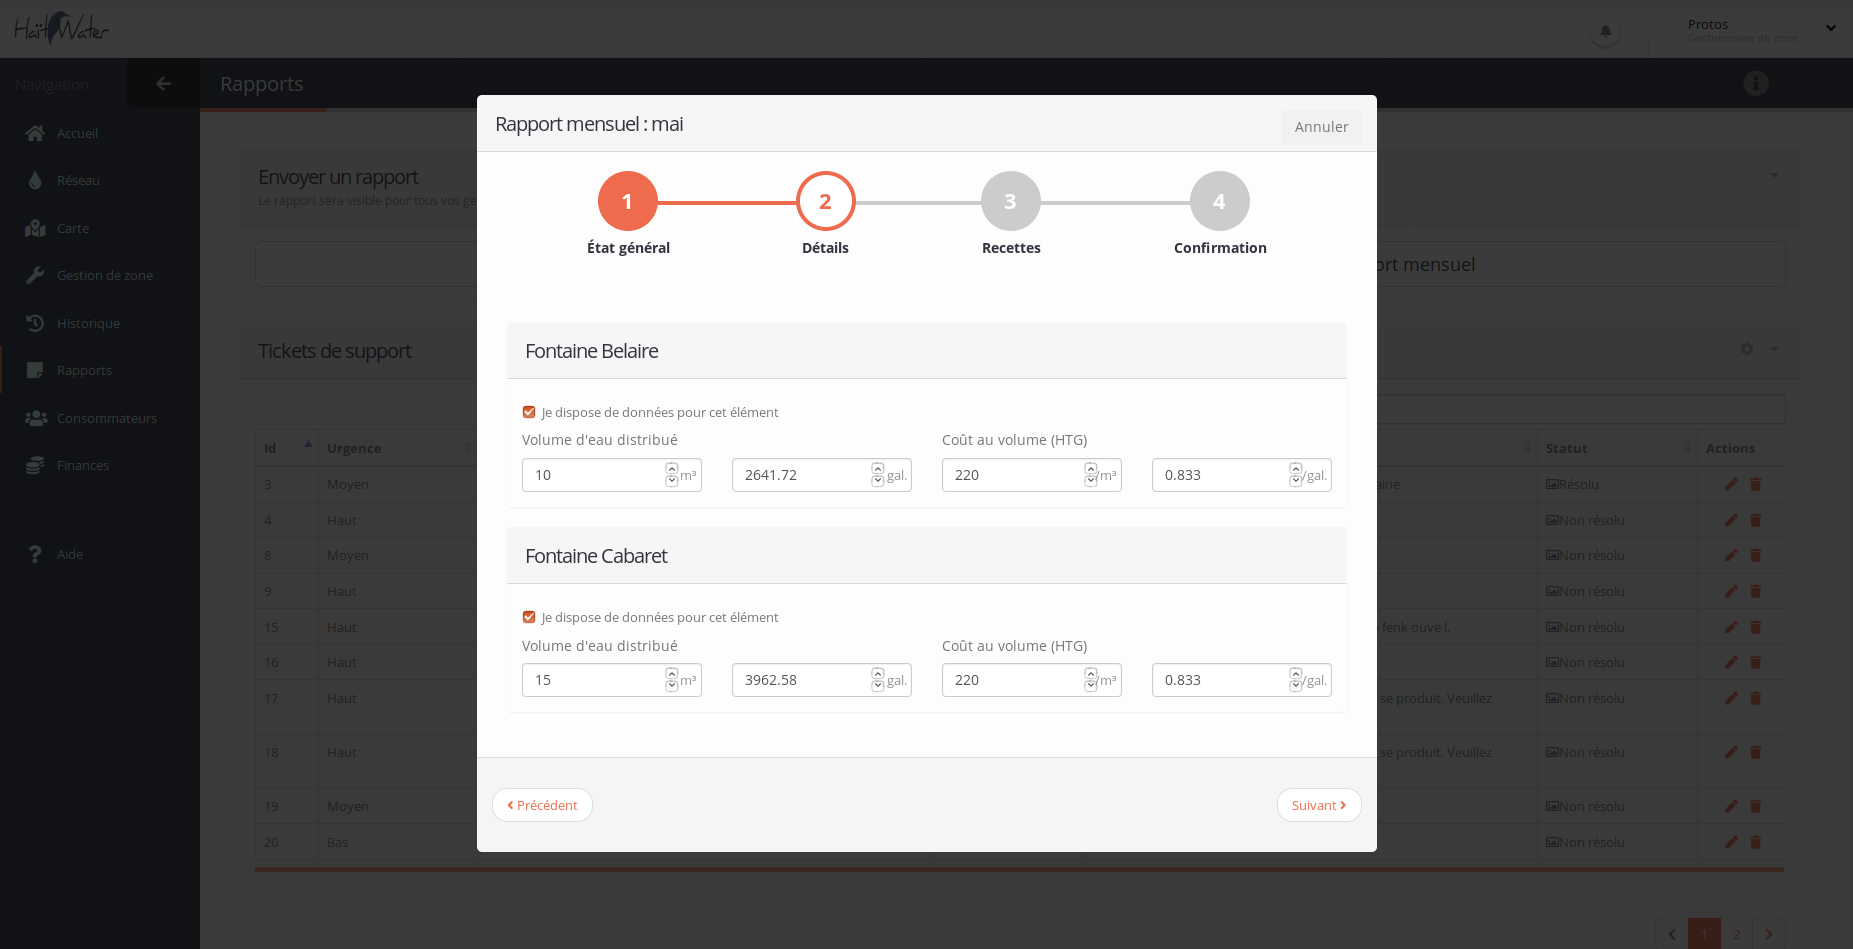
\includegraphics[width=\textwidth]{images/screen_rapport_mensuel.png}
				\caption{Capture d'écran du formulaire de rapport mensuel d'HaïtiWater}
				\label{fig:screen_rapport_mensuel}
			\end{figure}

			Ces formulaires ont pour objectif d'accompagner l'utilisateur dans ses tâches. En figure~\ref{fig:screen_rapport_mensuel}, vous observez que pour atteindre ce but, nous mettons en place un formulaire qui se consulte de haut en bas et de droite à gauche, où chaque information entrée est une information qui ne nécessite aucun retour en arrière. Sur ce formulaire en particulier, l'utilisateur peut entrer des données dans l'unité de volume de son choix (mètres cubes, gallons), la conversion est faite automatiquement. On trouve un autre exemple de ce genre d'accompagnement dans ce même formulaire, qui est séparé en quatre parties distinctes. Celles-ci qui évitent un bloc formulaire trop grand et permettent une transition entre différentes parties logiques du rapport mensuel.

			%TODO voir si on met les screens de toute l'application en annexe

		\section{Procédure d'utilisation}

			%Pages : 2 à 3

			%TODO que mettre en contenu ? à voir avec le CdC

		\section{Client}

			% Le client est la partie visible de l'iceberg. Quand même un gros morceau mais totalement inutile sans le back. Il y a des calculs et conversions effectuées pour alléger la connexion, mais aucun calcul n'est enregistré en back (don't trust the user).
			L'interface et sa facilité d'utilisation n'a pas été le seul axe du développement du client. C'est au niveau technologique que nous trouvons deux contraintes importantes : l'allégement de l'utilisation de la connexion et la simplification du code source derrière l'application.

			\subsection*{Mise en cache}
				\label{sec:cache_client}

				La mise en cache est un système natif commun à la vaste majorité des navigateurs modernes. Le concept est simple; conserver l'ancienne version d'un fichier pour la réutiliser la prochaine fois si elle n'a pas changé. HaïtiWater utilise pleinement ce concept pour alléger le poids des téléchargements. Nous avons poursuivi un objectif de généricité dans le code source afin d'éliminer la redondance et de permettre une forte réutilisation des composants. Grâce à cette mise en cache, les pages de l'application qui font en moyenne $1,2$MB lors de la première visite ne requierent qu'approximativement $10$KB de téléchargement pour les suivantes. Une exception peut être notée; le module d'information géographique est plus gourmand en ressources réseau en raison du téléchargement des images composant la carte.

			%Pages : 4 à 5
			\subsection*{Gabarits, modularité et responsiveness}
				% Interface construite en blocs (screen?)
				Nous avons vu plus tôt que l'application est constituée d'une zone de travail dans laquelle des blocs de contrôles sont placés pour former les différents modules de l'application. Ces blocs de contrôle reflètent l'architecture logicielle de l'interface.

				Pour implémenter ces contrôles, nous utilisons les gabarits Django qui sont des blocs de code HTML établissant la structure de la page web. Ces différents blocs de structure sont ensuite utilisés dans l'application pour créer les différentes pages :
				\begin{itemize}
					\item En \emph{extension}, c'est-à-dire que nous crééons une nouvelle page à partir d'un gabarit existant. Les contrôles communs (figure~\ref{fig:capture_gis}.1-3) de l'application sont ainsi définis une seule fois et réutilisés à travers les modules.
					\item En \emph{inclusion}, dans laquelle un bloc de contrôle est défini indépendamment d'une page, lui permettant de conserver le même fonctionnement en une seule implémentation à travers plusieurs pages web. Les tables et formulaires sont des exemples typiques.
				\end{itemize}



			\subsection*{Accessibilité hors-ligne}
				\label{sec:service_worker}

				Une contrainte importante en Haïti est la disponibilité de la connexion internet. Dès lors, il est nécessaire pour les futurs utilisateurs de notre application de pouvoir y accéder hors ligne. Cela n'est d'habitude pas possible pour un site internet, cependant la fondation Mozilla a développé récemment les Services Workers \cite{ref:serviceworker}. Il s'agit d'un module qui s'ajoute sur la machine de l'utilisateur et vient intercepter les requêtes effectuées par le client avant qu'elles ne soient transmises au serveur, afin d'y effectuer différents traitements.

				L'une des capacités du Service Worker est de coordonner la mise en cache des documents renvoyés par le serveur sur le navigateur internet de l'utilisateur. Initialement, le cache est vide. Lorsqu'une requête pour un document est reçue, il est stocké dans ce cache par le Service Worker. Par la suite, les prochaines requêtes pour ce document seront interceptées par ce module, qui ira chercher les informations directement dans le cache du navigateur à la place de transférer la requête au serveur.

				Il est également possible d'intercepter les requêtes faites au serveur lorsque celui-ci n'est pas accessible, comme lorsque la connexion internet n'est pas stable. De cette manière, nous pouvons quand même offrir certaines fonctionnalités hors-connexion. Cependant, il est encore nécessaire de choisir quelles fonctionnalités proposer dans ce cas. Le Service Worker se trouvant sur la machine de l'utilisateur ne peut utiliser que les données qui lui sont accessibles puisque le serveur n'est pas disponible. Pour cela, nous avons imaginé trois choix possibles :

				\begin{itemize}
					\item Toutes les fonctionnalités. Cela implique d'avoir une version locale de la base de données sur la machine de l'utilisateur. Il est aussi nécessaire de synchroniser les différentes versions de celle-ci, y compris en cas d'inconsistance, si deux utilisateurs déconnectés modifient le même élément par exemple.
					\item Version statique des données. Cela implique également d'avoir une version locale de la base de donnée, mais en supprimant la possibilité de modifier ces données sans connexion. Cela simplifie la synchronisation et règle les problèmes d'inconsistance.
					\item Quelques formulaires d'ajout. En retirant la possibilité de visualiser des données, il n'est dès lors pas nécessaire de garder une base de donnée sur la machine de l'utilisateur. Les fonctionnalités restantes sont la possibilité de remplir des formulaires d'ajout pour différentes tables, ce qui nous semble être la tâche la plus importante à avoir lorsqu'il n'y a pas de connexion, afin de ne pas perdre d'informations.
				\end{itemize}

				Nous nous sommes finalement décidés pour cette dernière option, qui nous semblait plus réaliste et plus en accord avec la faible connexion d'Haïti. Il est dès lors possible pour un utilisateur de compléter le rapport mensuel hors connexion. Ce module est facilement extensible à la possibilité de compléter d'autres formulaires dans le futur, voire à la possibilité d'accéder aux données s'il apparaît que cette fonctionnalité est importante pour les utilisateurs finaux de l'application.

				Au final, les Services Workers nous permettent d'avoir des fonctionnalités autrement impossible sur un site web. Ils ont aussi l'avantage d'être un standard maintenant disponible sur tous les navigateurs majeurs. Cependant, cette compatibilité est relativement récente et des utilisateurs utilisant de vieilles versions de ces navigateurs risquent de ne pas avoir accès à cette technologie. Heureusement, cette fonctionnalité est entièrement optionnelle et le site fonctionne encore sans cette compatibilité. Il est également possible pour tout utilisateur de simplement mettre à jour ou changer de navigateur, s'il venait à avoir besoin des Service Workers.

			\subsection*{...}

		\section{Serveur}
			\label{sec:serveur}

			% Parler de l'API, pourquoi c'est bien à la place d'utiliser du django classique et comment on l'a faite
			% Parler de l'ORM de Django

			Pages : 4 à 5
			\subsection*{Authentification}
			\subsection*{Requêtes}
			\subsection*{...}

	\chapter{Validation}

		%Total des pages : 8 à 11
		La validation rassemble les étapes du projet qui ont pour but de vérifier le fonctionnement et la qualité des productions. Les premières validations se sont essentiellement basées sur des productions écrites (cahier des charges, schémas) présentées aux acteurs d'Haïti, à Protos et à nos promoteurs pour exposer notre avancement et l'orientation du travail futur.

		\section{Performances}

			Pages : 3 à 4

			\subsection*{Temps}
			\subsection*{Poids}

		\section{Vérifications automatiques}
			%TODO Sébastien
			Pages : 2 à 3

			\subsection*{Tests unitaires}
			\subsection*{Tests fonctionnels} % TODO See if done

		\section{Vérifications utilisateurs réels}
			% Pages : 3 à 4
			Cette étape, qui s'est déroulée de mars à avril, a mis des utilisateurs étrangers à l'équipe de développement face à l'application. Derrière cette vérification, deux points de l'application étaient mis à l'épreuve : l'interface graphique et la procédure d'utilisation. Après plusieurs mois de développement, le point de vue d'utilisateurs externes avec des connaissances en informatique et en gestion de l'eau fortement variables était nécessaire.

			Les séances de validation ont eu lieu selon les disponibilités des utilisateurs d'essai, répartis en deux groupes. Un premier groupe de 9 utilisateurs a testé l'application dans la version \emph{Alpha 3}, un second groupe de 11 utilisateurs a testé l'application dans la version \emph{Beta 1}, dans laquelle les modules financier et historique ont été rajoutés ainsi que plusieurs changements suggérés par les utilisateurs d'essai du premier groupe de validation.

			\subsection*{Méthodologie}

				Afin d'introduire un minimum d'erreurs statistiques, la mesure de la satisfaction des utilisateurs a suivi un protocole (protocole complet disponible en annexe~\ref{sec:documents_validation}) établi avec l'expérience de nos promoteurs sur base d'un ancien travail de fin d'études~\cite{ref:reflecton}, de cours~\cite{ref:vanderdonckt_hci, ref:vanderdonckt_cscw} et recherches sur la satisfaction utilisateur~\cite{ref:usability_evaluation_tools, ref:ssi}.

				Autant que possible, les séances se sont déroulées en présence physique de l'utilisateur d'essai. Certaines contraintes horaires et logistiques ont imposé la réalisation de séances à distance dans lesquelles nous avons utilisé Skype ou Discord, logiciels permettant de transmettre la voix et partager l'écran de l'utilisateur.

				Après une brève introduction au concept de l'application et aux objectifs de la séance, les utilisateurs obtiennent un scénario composé d'un contexte et de tâches à réaliser qu'ils peuvent lire à leur aise. Un utilisateur travaille seul et est chronométré durant la séance. S'il a une question ou s'il reste bloqué sur une tâche, un indice lui est donné et noté dans un document avec le temps nécessité pour réaliser la tâche.

				Après trois scénarios accomplis, l'utilisateur d'essai remplit un formulaire (Google Form\copyright) anonymisé composé de 24 questions fermées réparties en quatre sections :
				\begin{description}
					\item[Général] est une première section cherchant à identifier si l'utilisateur a compris les tâches qu'il vient d'accomplir avec l'application.
					\item[Fonctionnalités] cherche à identifier la compréhension des contrôles de l'application par l'utilisateur.
					\item[Usabilité] est une section particulière. Composée de dix questions alternant des assertions positives et négatives en alternance, cette section est une transcription en français de la \emph{System Usability Scale (SUS)}~\cite{ref:sus}. Se décrivant comme une mesure rapide et sâle, la SUS présente l'avantage de pouvoir être complétée rapidement par nos utilisateurs d'essai durant ces séances de maximum deux heures non-rémunérées.
					\item[Esthétique] est une dernière section, sans doute la plus subjective, composée de questions sur l'apparence de l'interface graphique.
				\end{description}

				L'utilisateur sélectionne la réponse sur une échelle de Likert~\cite{ref:wikipedia_likert_scale} à 5 valeurs allant de \emph{Pas du tout d'accord} à \emph{Tout à fait d'accord}. Si l'utilisateur ne comprend pas la question ou n'a pas d'avis, il sélectionne le \emph{neutre}.

			\subsection*{Résultats obtenus}

				Les contraintes inhérentes au cadre du mémoire, principalement en temps et budget, nous empêchent de pouvoir réaliser une étude qui donnerait une mesure plutôt précise de la satisfaction utilisateur. Néanmoins, de nos vingt réponses des utilisateurs d'essai nous pouvons tout de même extraire une certaine indication de l'expérience utilisateur d'HaïtiWater.

				Les résultats des 14 questions évaluant la satisfaction des utilisateurs sur le concept, les fonctionnalités et l'esthétique de l'application sont représentés en figure~\ref{fig:validation_likert}.

				\begin{figure}[H]
					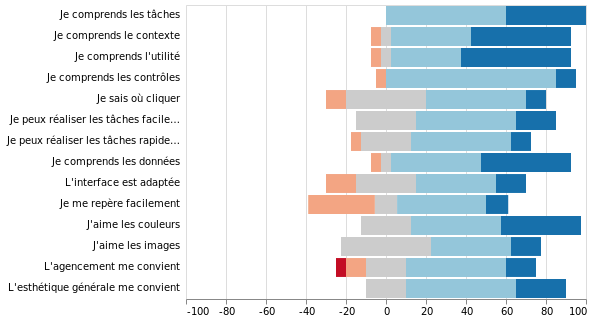
\includegraphics[width=\textwidth]{images/likert_questions}
					\caption{Répartition des réponses aux questions du formulaire de validation}
					\label{fig:validation_likert}
				\end{figure}

				Nous pouvons constater une tendance positive dans les réponses aux questions ainsi qu'une cohérence dans les groupements : les quatre questions ayant reçu le score le plus bas sont toutes liées à une certaine complexité de l'interface.

				Les dix questions de la SUS s'évaluent différemment. L'échelle a sa propre formule de calcul~\cite{ref:sus} qui permet de normaliser les résultats à une valeur de 0 à 100. Notez cependant qu'il ne s'agit pas d'un pourcentage de qualité mais d'une valeur suivant une distribution gaussienne dont la moyenne empirique se situe à 68. Le premier groupe de validation nous plaçait à 67,5, le second à 77,5 pour une moyenne à 73. Nous devons rester précautionneux quant à ces résultats, mais ils montrent que l'interface est plutôt bien reçue. L'augmentation des résultats entre les deux groupes est positive et montre que les changements déjà apportés à l'application après le premier groupe ont eu un impact positif sur l'expérience utilisateur.

			\subsection*{Modifications apportées}
				% TODO Adrien mods + module "aide"

	\chapter{Améliorations futures}

		Total des pages : 4 à 7

		\section{Suite du projet}
			\label{ref:suite_projet}
			% Lors du déploiement, même si le site est pas hyper lourd, on peut encore l'alléger en faisant du coverage par les navigateurs (quelques stats), pas une bonne idée de le faire maintenant vu que développement pas fini.

			Pages : 2 à 3

		\section{Défis rencontrés}

			Pages : 1 à 2

		\section{Propositions}

			Pages : 1 à 2

	\chapter{Conclusion}

		Pages : 1 à 2

	\chapter*{Bibliographie}
	\addcontentsline{toc}{chapter}{Bibliographie}

	\bibliography{bibliography}{}
	\bibliographystyle{plain}

		Pages : 2 à 3

	\appendix

	\chapter{Cahier des charges complet}

		Pages : beaucoup

	\chapter{Base de données}

		Pages : beaucoup

	\chapter{Wireframes}
		\label{sec:wireframes}
		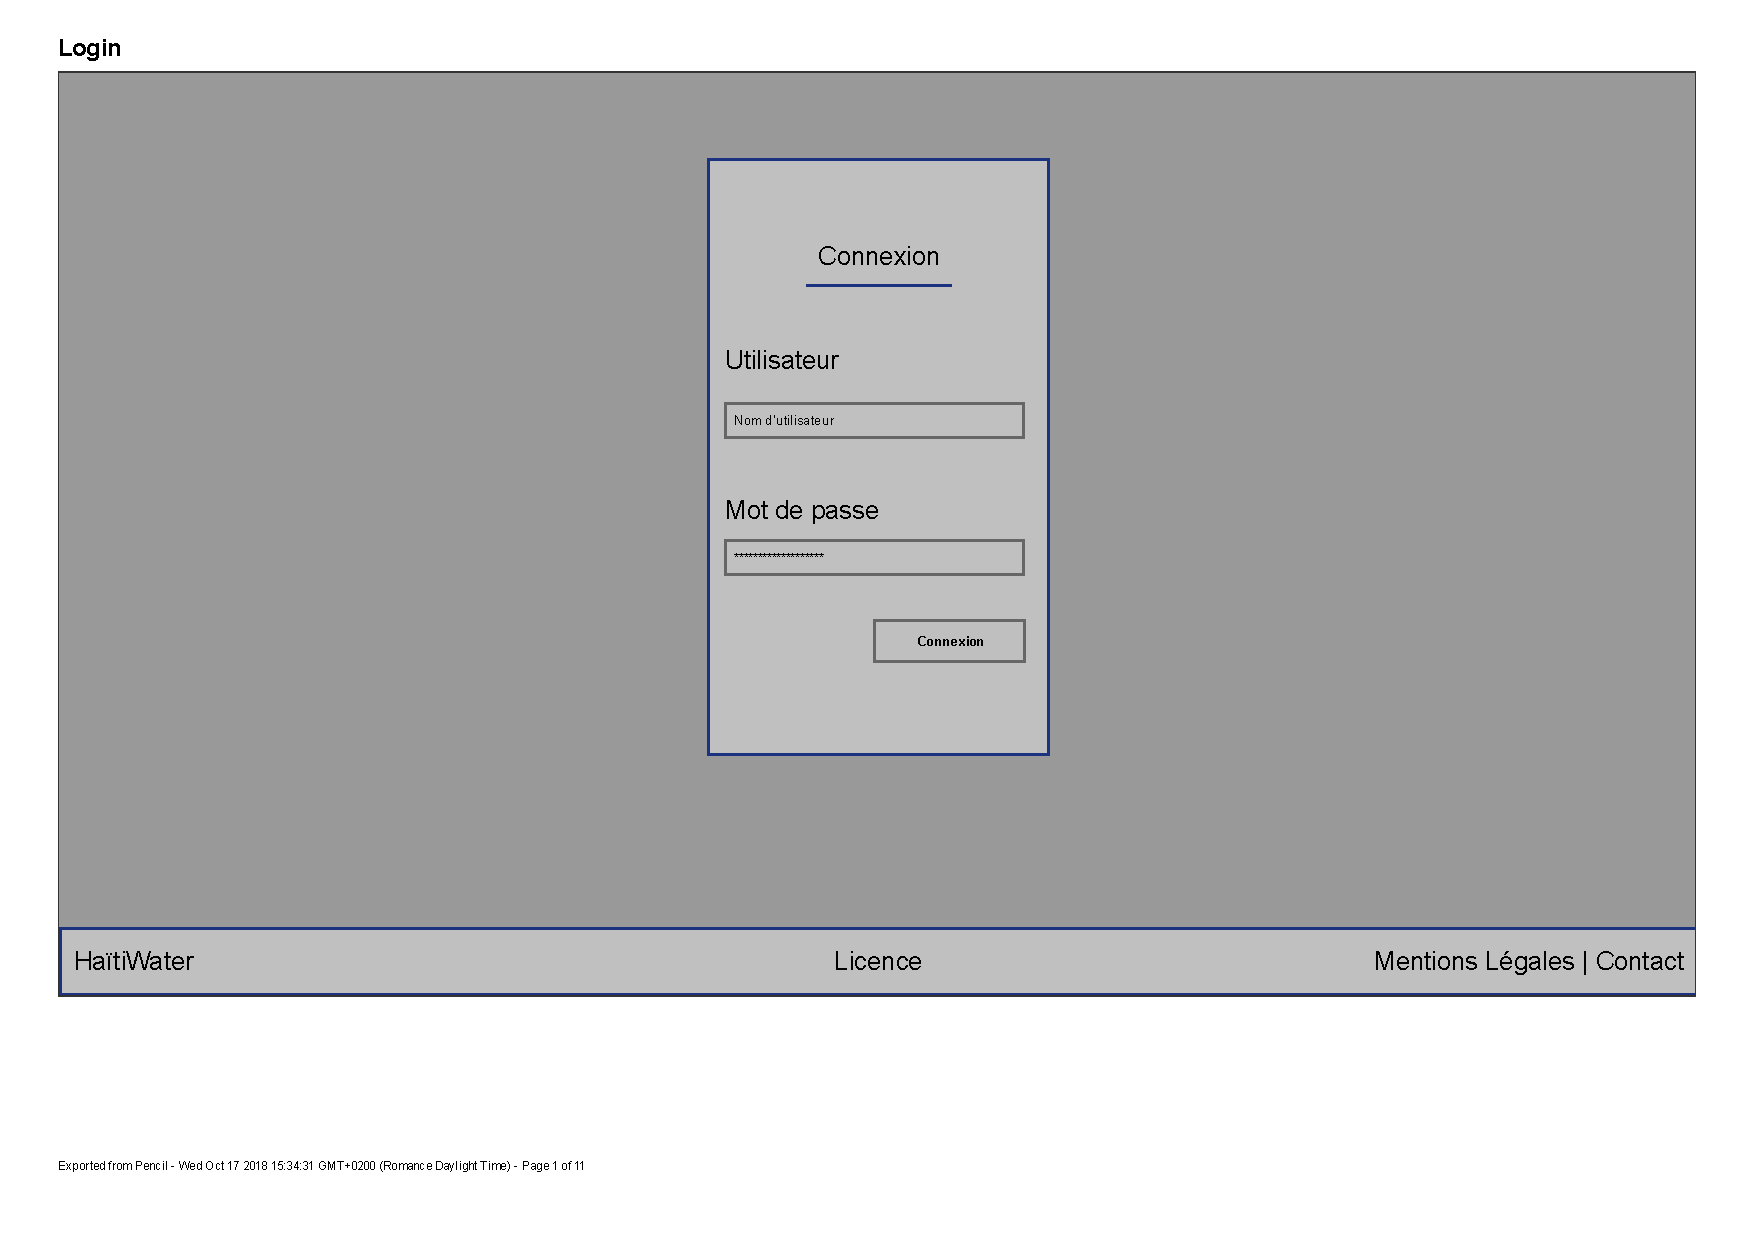
\includepdf[pages=-,nup=1x2,pagecommand={},width=\textwidth]{../documents/design/wireframes/hi-fi/wireframes_hifi_pencil.pdf}

	\chapter{Diagrammes d'activité}

		Pages : beaucoup

	\chapter{Documents de validation}
		\label{sec:documents_validation}
		\section*{Abstract}
    Ce document établit le protocole et les questions de l'expérience de validation de l'interface et des fonctionnalités de l'application, principalement du point de vue de la facilité d'utilisation et de compréhension, avec des utilisateurs hors de l'équipe de développement. En fin de document, vous trouvez les scénarios tels que les utilisateurs les verront imprimés lors des essais.
\hrule

\section{Objectifs}
    Les expériences de validation cherchent à mettre en avant les points forts/faibles de l'interface graphique en utilisant un protocole identique, pour plusieurs participants, visant à normaliser les résultats et tenter de dégager une tendance positive ou négative. Les résultats de l'expérimentation permettront de confirmer ou infirmer certains choix techniques, esthétiques et fonctionnels. L'exactitude des résultats n'est pas évaluée lors de cette validation.

\section{Protocole}
    \subsection*{Résumé}
        Chaque participant est introduit à l'application de manière générale sans présentation de l'interface. Chaque participant reçoit un numéro. L'expérimentation commence avec un scénario et un type d'interface (mobile ou desktop) défini. L'application est déjà ouverte sur le périphérique utilisé. Le participant doit ensuite compléter un scénario, divisé en plusieurs tâches, dans le temps imparti. Si le participant ne parvient pas à résoudre une tâche, il peut être aidé de manière brève et orale par l'expérimentateur qui notera chaque intervention de sa part. Une fois le scénario accompli, le participant réitère sur d'autres scénarios pour une durée maximale d'une heure trente au total. La dernière demie-heure est réservée à la complétion d'un formulaire en ligne composé de 24 questions utilisant une échelle de Likert~\cite{ref:wikipedia_likert_scale} et à une éventuelle discussion avec les participants.

    \subsection*{Présentation}
        L'objectif de l'application est de fournir un appui logiciel aux gestionnaires du réseau de distribution d'eau potable d'Haïti. On considère qu'il y a deux groupes d'utilisateurs principaux:
        \begin{itemize}
            \item Le \emph{gestionnaire de zone} qui coordonne l'activité dans une certaine zone géographique. Il est un responsable administratif.
            \item Le \emph{gestionnaire de fontaine} qui participe au quotidien à la gestion physique du réseau de distribution. Il est au plus proche contact des consommateurs.
        \end{itemize}
        En tant que sujet d'expérimentation, le participant va être présenté à différentes situations qui vont lui demander d'utiliser l'application à divers degrés de responsabilité et à travers plusieurs écrans. Le participant reçoit un numéro permettant de l'identifier à travers les différents scénarios.

    \subsection*{Scénarios d'utilisation}
        L'utilisateur est placé devant l'application, ouverte sur le portail de connexion, et peut lire le scénario qui lui est proposé. Une fois prêt, l'utilisateur démarre la tâche et l'expérimentateur lance le chronomètre. Chaque participant est seul devant l'application ouverte en mode écran complet, écran simulant une tablette ou un smartphone. Le scénario (comprenant les instructions) lui est laissé à disposition. L'expérimentateur peut venir en aide au participant de manière brève et sans interagir avec le périphérique. Toute aide apportée sera notée. Une fois le scénario accompli, le temps écoulé est noté par l'expérimentateur. Si le participant ne parvient pas à compléter la tâche dans le temps imparti, l'expérimentateur interrompt l'expérience.

        Après un scénario accompli, le participant peut en commencer un nouveau. Les scénarios sont choisis aléatoirement.

    \subsection*{Questionnaire}
        Après accomplissement des tâches, le participant complète le questionnaire annexe visant à évaluer sa satisfaction quant à l'utilisation du logiciel et composé des 24 questions ci-après et d'un commentaire libre. Les questions sont regroupées en catégories. Chaque question dispose
        de quatre choix à sélection unique basés sur une échelle de Likert~\cite{ref:wikipedia_likert_scale}: \texttt{-{}-}, \texttt{-}, Neutre, \texttt{+} et \texttt{++}.
        La section usabilité se base sur la \emph{Software Usability Scale}~\cite{ref:sus, ref:usability_evaluation_tools}, qui est une technique d'évaluation simple et rapide de l'usabilité, traduite et adaptée au contexte de l'application. Les participants doivent répondre sans trop réfléchir aux questions et de manière individuelle. Si un participant ne peut répondre à une question, il doit sélectionner le neutre comme demandé par la software usability scale. Les autres sections se basent sur des gabarits d'évaluation logicielle~\cite{ref:ssi} et expérimentations précédentes~\cite{ref:reflecton}. En plus d'un commentaire libre final, chacune des quatre sections de questions dispose d'un champ de commentaire libre.

        \subsection*{Général}
            \begin{description}
                \item[G1] Je comprends les tâches demandées.
                \item[G2] Je comprends l'utilité des tâches demandées dans le contexte de la gestion de l'eau.
                \item[G3] Je comprends l'utilité de l'application.
            \end{description}
        \subsubsection*{Fonctionnalités}
            \begin{description}
                \item[F1] Je comprends l'utilité des contrôles de l'interface, je sais à quoi m'attendre en utilisant un contrôle (bouton, champ de texte, ...).
                \item[F2] Je sais où cliquer pour réaliser la tâche demandée.
                \item[F4] Je peux réaliser les tâches facilement.
                \item[F5] Je peux réaliser les tâches rapidement.
                \item[F6] Je comprends les données qui me sont présentées à l'écran.
                \item[F7] L'interface de l'application est adaptée aux tâches demandées.
                \item[F8] Je sais me repérer facilement dans les contrôles et menus de l'application.
            \end{description}

        \subsection*{Usabilité}
            \begin{description}
                \item[U1] Je pense que j'aimerais utiliser l'application fréquemment.
                \item[U2] Je trouve l'application inutilement complexe.
                \item[U3] Je trouve l'application facile à utiliser.
                \item[U4] J'aurais besoin de l'aide d'une personne qualifiée pour utiliser ce système.
                \item[U5] J'ai trouvé les différentes fonctionnalités du système bien intégrées.
                \item[U6] J'ai trouvé l'application trop inconsistante.
                \item[U7] Je pense que la plupart des utilisateurs apprendraient à utiliser l'application rapidement.
                \item[U8] J'ai trouvé l'application très lourd à utiliser.
                \item[U9] Je suis confiant en utilisant l'application.
                \item[U10] J'ai besoin d'apprendre beaucoup de choses avant de pouvoir utiliser l'application.
            \end{description}

        \subsection*{Esthétique}
            \begin{description}
                \item[E1] J'aime les couleurs de l'application.
                \item[E2] J'aime les images de l'application.
                \item[E3] L'agencement visuel (position des éléments) de l'application me convient.
                \item[E4] L'esthétique générale de l'application me satisfait.
            \end{description}

\section{Attentes}
    Avec cette expérimentation, nous cherchons à obtenir des vues externes sur l'application et ses fonctionnalités, récoltées de manière rigoureuse afin d'être critiques et objectifs quant aux réalisations logicielles. La phase de validation arrivant avant la phase de documentation finale, nous espérons non seulement récolter des informations sur la qualité de l'application sans documentation, mais aussi sur les points importants de la documentation et sur lesquels il faudra insister. Les objectifs sont donc de déceler les problèmes et d'envisager leurs solutions, dans l'objectif de les mettre en place dans la documentation utilisateur ou dans le logiciel (selon des critères d'utilité, expérience utilisateur et pertinence).

\newpage
\section*{Scenario 1 - Gestion}
    \begin{description}
        \item[Rôle] Administrateur principal
        \item[Objectif] Créer une nouvelle zone et y assigner un gestionnaire
        \item[Prérequis du système] /
        \item[Contexte] Vous êtes Claude, membre de l’ONG Protos. L’application HaïtiWater est déjà utilisée dans plusieurs départements d’Haïti et le département de l’Artibonite souhaite pouvoir l’utiliser également. En tant que responsable de l’application, vous devez permettre au responsable de la gestion de l’eau en Artibonite de se connecter à l’application et de gérer son réseau. Pour que le réseau de l’Artibonite soit indépendant des autres réseaux, vous devez créer une nouvelle zone et y assigner le responsable de la gestion de l'eau en Artibonite.
    \end{description}

    \subsubsection*{Informations nécessaires}
        \begin{multicols}{2}
            Vos informations:
            \begin{description}
                \item[Utilisateur] Protos
                \item[Mot de passe] Protos
            \end{description}
            \vfill\null
            \columnbreak

            Gestionnaire en Artibonite:
            \begin{description}
                \item[Nom] Registre
                \item[Prénom] Jean
                \item[Courriel] haitiwater.test@gmail.com
            \end{description}
        \end{multicols}

    \subsubsection*{Tâches (30 minutes)}
        \begin{enumerate}
            \item Connectez-vous à l'application avec votre compte de gestionnaire: Protos.
            \item L’Artibonite n’existe pas encore dans l'application, vous devez l’ajouter en tant que nouvelle zone. Pour cela, il faut aller dans l’onglet de gestion de zone et créer une nouvelle zone. Vous pouvez choisir son nom.
            \item Maintenant que l’Artibonite existe en tant que zone, vous devez y assigner un gestionnaire pour que le réseau puisse s’y développer. Ajoutez donc Jean Registre en tant que gestionnaire de cette nouvelle zone afin qu’il puisse se connecter à l’application.
            \item Quittez l’application en vous déconnectant pour revenir à l’écran d’accueil.
        \end{enumerate}
\newpage

\section*{Scenario 2 - Utiliser les tables}
    \begin{description}
        \item[Rôle] Gestionnaire de zone
        \item[Objectif] Imprimer la liste des tous les éléments (fontaines, kiosques, ...) du réseau de la zone \emph{CAEPA Passe Catabois} classées par volume de sortie total
        \item[Prérequis du système] Plusieurs avec plus de dix fontaines par zone, ou la version live du serveur.
        \item[Contexte] Vous êtes Dominique, gestionnaire de zone et supervisez les opérations au niveau national. Cette semaine, une réunion a lieu pour décider des budgets alloués à la maintenance des fontaines de la zone de l'Ouest. Pour vous aider à allouer les fonds de manière équitable, vous avez besoin de la liste des installations de cette zone, classées par nombre d'utilisateurs décroissant.
    \end{description}

    \subsubsection*{Informations nécessaires}
        Vos informations:
        \begin{description}
            \item[Utilisateur] Protos
            \item[Mot de passe] Protos
        \end{description}
    \subsubsection*{Tâches (30 minutes)}
        \begin{enumerate}
            \item Connectez-vous à l'application avec vote compte de gestionnaire: Protos.
            \item Rendez-vous dans votre page de gestion et trouvez un moyen de filtrer les éléments pour ne conserver que ceux de la zone  \emph{CAEPA Passe Catabois}.
            \item Triez les éléments par nombre d'utilisateurs décroissant.
            \item Imprimez les éléments en vous assurant d'avoir la liste complète affichée. Par défaut, les tables n'affichent qu'un nombre limité d'éléments (10). Vous pouvez vous arrêter une fois que le navigateur vous propose d'imprimer le bon document, il n'est pas nécessaire de l'imprimer physiquement.
        \end{enumerate}

\newpage

\section*{Scenario 3 - Gestionnaire de fontaine}
    \begin{description}
        \item[Rôle] Gestionnaire de fontaine
        \item[Objectif] Ajouter des consommateurs et envoyer un rapport mensuel
        \item[Prérequis du système] Un gestionnaire de fontaines et ses éléments du réseau: une fontaine, un kiosque et une prise individuelle.
        \item[Contexte] Vous êtes Frédérique, gestionnaire de fontaine. Vous avez la responsabilité de trois points d'eau et d'une communauté d'utilisateurs. Votre objctif de la journée est d'enregistrer un nouveau consommateur ayant récemment déménagé dans la région, puis d'envoyer votre rapport mensuel.
    \end{description}

    \subsubsection*{Informations nécessaires}
    \begin{multicols}{2}
        Vos informations:
        \begin{description}
            \item[Utilisateur] frederique
            \item[Mot de passe] gestionfontaine
        \end{description}
        \vfill\null
        \columnbreak

        Le nouveau consommateur est Monsieur Alain Proviste. Il vit seul au 32, Rue du foin, Belleville. Nous n'avons pas son numéro de téléphone et il habite juste à côté de la seule fontaine du village.
    \end{multicols}

    \subsubsection*{Tâches (30 minutes)}
        \begin{enumerate}
            \item Connectez-vous sur l'application avec votre compte.
            \item Ajoutez le nouveau consommateur récemment arrivé
            \item Envoyez le rapport du mois en cours
            Informations mensuelles:
            \begin{description}
                \item[Activité] 22 jours, 14 heures par jour.
                \item[Kiosque] 400 gallons de volume total à 10 gourdes le gallon
                \item[Fontaine] 2 mètres cubes de volume total à 500 gourdes le mètre cube
                \item[Prise individuelle] un demi mètre cube à 500 gourdes le mètre cube
                \item[Recettes] 0 gourdes pour le kiosque et la fontaine, 150 gourdes pour la prise individuelle
            \end{description}
            \item Déconnectez-vous de l'application
        \end{enumerate}

\newpage

\section*{Scenario 4 - Système d'Informations Géographiques}
    \begin{description}
        \item[Rôle] Gestionnaire de zone
        \item[Objectif] Dessiner une partie du réseau sur la carte
        \item[Prérequis du système] Connecté et sur la page d'accueil. Aucun élément dans le système.
        \item[Contexte] Vous êtes le gestionnaire d'une zone nouvellement établie. Avant de créer les gestionnaires de fontaine qui vont vous aider dans votre travail, vous souhaitez avoir votre réseau encodé dans l'application. Vous allez donc prendre un peu de temps pour ajouter les éléments un par un dans le système et sur la carte.
    \end{description}

    \subsubsection*{Informations nécessaires}
        Votre réseau de distribution de l'eau potable est composé de:
        \begin{description}
            \item[Une source] qui pompe l'eau dans le circuit. Elle est située dans le lieu-dit \emph{Cabaret}. Nous avons les coordonnées précises: 19\textdegree 33'56.6"N, 72\textdegree 00'32.5"W.
            \item[Une fontaine] dont nous n'avons pas les coordonnées mais qui se situe en aval de la rivière, sur la route au premier carrefour après la pompe.
            \item[Une conduite] qui relie les deux.
        \end{description}

    \subsubsection*{Tâches (30 minutes)}
        \begin{enumerate}
            \item Vous êtes sur la page d'accueil, rendez-vous sur la page de gestion géographique du réseau.
            \item Créez la source \emph{Cabaret} dans les éléments du réseau et ajoutez sa position via ses coordonnées géographiques.
            \item Créez la fontaine du carrefour dans la base de données, et placez-la sur la carte, utilisez la source déjà placée pour trouver le prochain carrefour au nord.
            \item Créez une conduite dans les éléments, et placez la sur la carte pour relier les deux autres éléments que vous venez de créer.
            \item Une fois que les trois éléments sont encodés dans la base de données et placés sur la carte, déconnectez-vous.
        \end{enumerate}

\newpage

\section*{Scenario 5 - Première connexion et problème}
    \begin{description}
        \item[Rôle] Gestionnaire de fontaine
        \item[Objectif] Se connecter pour la première fois, changer de mot de passe et signaler un problème
        \item[Prérequis du système] Un utilisateur avec un mot de passe autogénéré et un élément
        \item[Contexte] Vous êtes Jean, un gestionnaire de fontaine nouvellement nommé, félicitations ! Vous venez à l'instant de recevoir un courriel vous donnant vos informations de connexion. Le mot de passe généré est impossible à retenir alors vous allez le modifier. Vous allez également en profiter pour rapporter un problème mineur: votre fontaine produit des sons étranges quand on arrête de pomper.
    \end{description}

    \subsubsection*{Informations nécessaires}
    Vos informations:
    \begin{description}
        \item[Utilisateur] GestionnaireFontaine
        \item[Mot de passe] [Donné par l'examinateur]
    \end{description}

    \subsubsection*{Tâches (30 minutes)}
        \begin{enumerate}
            \item Connectez-vous à l'application à l'aide de votre mot de passe autogénéré.
            \item Modifiez votre mot de passe. Vous adorez le mot de passe "123456".
            \item On dirait qu'il y a un problème avec votre mot de passe. Trouvez une solution.
            \item Reconnectez-vous sur l'application avec votre nouveau mot de passe.
            \item Rapportez le problème décrit dans le contexte afin que votre hiérarchie en soit informée.
        \end{enumerate}

\newpage

\section*{Scenario 6 - Transaction financière}
    \begin{description}
        \item[Rôle] Gestionnaire de zone
        \item[Objectif] Se connecter et ajouter des paiements pour deux consommateurs.
        \item[Prérequis du système] Deux consommateurs dans la zone utilisateur (noms ci-dessous).
        \item[Contexte] Vous êtes John, un membre de l'administration du système HaïtiWater. En visite dans un village, vous en profitez pour aider un gestionnaire de fontaine local dans son encodage des paiements. Deux consommateurs viennent vous voir, billets en main, et viennent payer leur redevance.
    \end{description}

    \subsubsection*{Informations nécessaires}
    Vos informations:
    \begin{description}
        \item[Utilisateur] Protos
        \item[Mot de passe] Protos
    \end{description}

    \subsubsection*{Tâches (30 minutes)}
        \begin{enumerate}
            \item Connectez-vous à l'application à l'aide de vos informations.
            \item Rendez-vous dans la gestion financière de l'application.
            \item \emph{Monsieur Sadrac Mérisier} vous donne 150 Gourdes, entrez ce paiement dans l'application.
            \item \emph{Madame Roselène Monestime} vous donne 100 Gourdes, faites de même.
            \item A sa demande, informez \emph{Madame Roselène Monestime} de l'état général de ses paiements (dites à votre examinateur à combien de Gourdes s'élève son retard ou son avance sur les paiements).
            \item Déconnectez-vous de l'application.
        \end{enumerate}

	\setlength{\parskip}{0em}
	\backcoverpage

\end{document}
